\setcounter{chapter}{5}
\chapter{Folhas para reprodução}

\section{Lição 1}

\noindent {\bf Atividade 1} 
\vspace{.2cm}


\begin{tikzpicture}[scale=21]
 \draw[fill=brown] (0,0) rectangle (4.5,2); 
\end{tikzpicture}


\begin{tikzpicture}[scale=21]
 \draw[fill=brown] (0,0) rectangle (4.5,2);
 \draw (1,0) -- (1,2);
 \draw (2.5,0) -- (2.5,2);
\end{tikzpicture}

\clearpage
\noindent {\bf Atividade 2}
\vspace{.2cm}


\includegraphics[width=500pt,keepaspectratio]{..//media/cap1/secoes/pngs_licao_01/ativ2_fig02.png}

\noindent {\bf Atividade 3}
\vspace{.2cm}

\begin{tikzpicture}[scale=10]
\fill[attention]  \foreach \x/\y in {36/72,108/144,180/212, 252/284, 324/360}{ (0,0) -- (\x-18:4) -- (\y-18:2)--(\x-18 +72:4) -- (0, 0)};
\draw  \foreach \x/\y in {36/72,108/144,180/212, 252/284, 324/360}{ (\x-18:4) -- (\y-18:2)--(\x-18 +72:4)};
\end{tikzpicture}

\pagebreak

\noindent {\bf Atividade 4}
\vspace{.2cm}

\pagestyle{empty}
 \begin{tikzpicture}[scale=1.4, x=1cm,y=1cm]
  \draw (0,0) rectangle (1,6);
  \draw (1,0) rectangle (2,6);
  \draw (2,0) rectangle (3,6);
  \draw (3,0) rectangle (4,6);
  \draw (5,0) rectangle (9,3);
  \draw (5,0) rectangle (9,6);
  \draw (5,0) -- (9,3);
  \draw (5,3) -- (9,6);
\end{tikzpicture}
\vspace{0.5cm}

\begin{tikzpicture}[scale=1.4, x=1cm,y=1cm]
  \draw (0,0) rectangle (4,1.5);
  \draw (0,1.5) rectangle (4,3);
  \draw(0,3) rectangle (4,4.5);
  \draw(0,4.5) rectangle (4,6);
  \draw(5,0) rectangle (9,3);
  \draw(5,0) rectangle (9,6);
  \draw(7,0) -- (7,6);  
\end{tikzpicture}


 \begin{tikzpicture}[scale=1.4, x=1cm,y=1cm]
  \draw (10,0) rectangle (14,3);
  \draw (10,3) rectangle (14,6);
  \draw(12,0) -- (12,3);
  \draw(10,4.5) -- (14,4.5);
  \draw(15,0) rectangle (19,3);
  \draw(15,3) rectangle (19,6);
  \draw(15,1.5) -- (19,1.5);
  \draw(15,3) -- (19,6);
\end{tikzpicture}
\vspace{0.5cm}

\begin{tikzpicture}[scale=1.4, x=1cm,y=1cm]
  \draw (10,0) rectangle (14,3);
  \draw (10,3) rectangle (14,6);
  \draw (12,0) -- (12,3);
  \draw (10,3) -- (14,6);
  \draw (15,0) rectangle (19,3);
  \draw (15,3) rectangle (19,6);
  \draw (15,0) -- (19,3);
  \draw (19,3) -- (15,6);
\end{tikzpicture}

\pagebreak

{\bf Atividade 9}
\vspace{.2cm}

%retângulos

\noindent
\begin{tikzpicture}[scale=2, x=1cm,y=1cm]
 \draw[fill=gray] (0,0) rectangle (3,2);
 \draw (3,0) rectangle (6,2) (3,-0.4) node{Figura 1};
\end{tikzpicture}

\noindent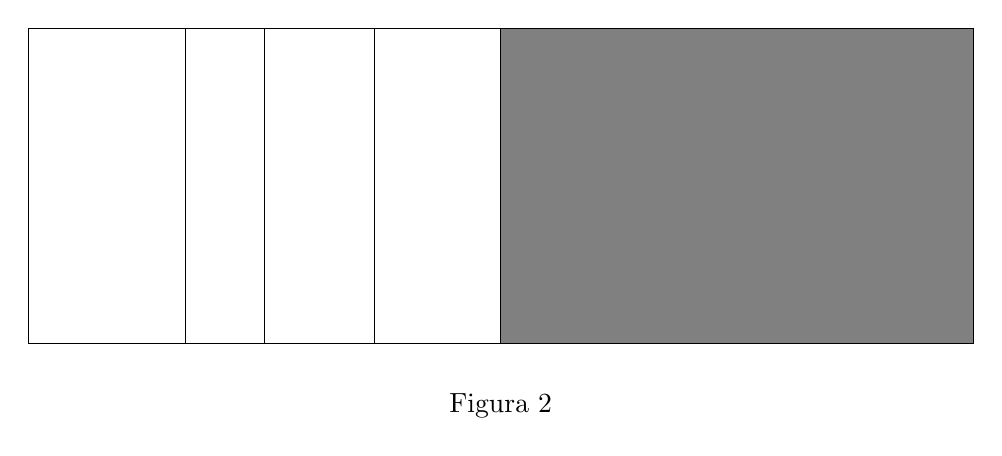
\begin{tikzpicture}[scale=2, x=1cm,y=1cm]
 \draw (0,0) rectangle (3,2);
 \draw (1,0) -- (1,2);
 \draw (1.5,0) -- (1.5,2);
 \draw (2.2,0) -- (2.2,2);
 \draw[fill=gray] (3,0) rectangle (6,2) (3,-0.4) node{Figura 2};
\end{tikzpicture}

\noindent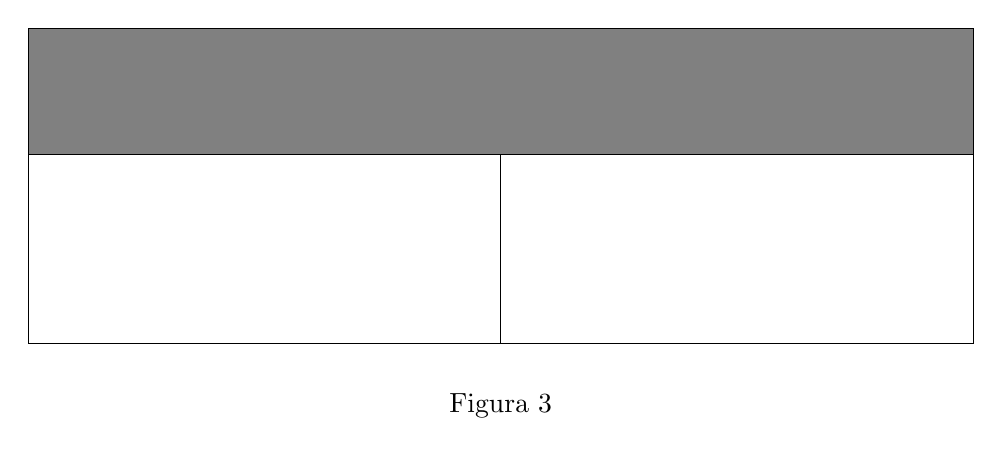
\begin{tikzpicture}[scale=2, x=1cm,y=1cm]
 \draw (0,0) rectangle (3,2);
 \draw (3,0) rectangle (6,2) (3,-0.4) node{Figura 3};
 \draw[fill=gray] (0,2) rectangle (6,1.2);
 \end{tikzpicture}

 % círculos

\noindent 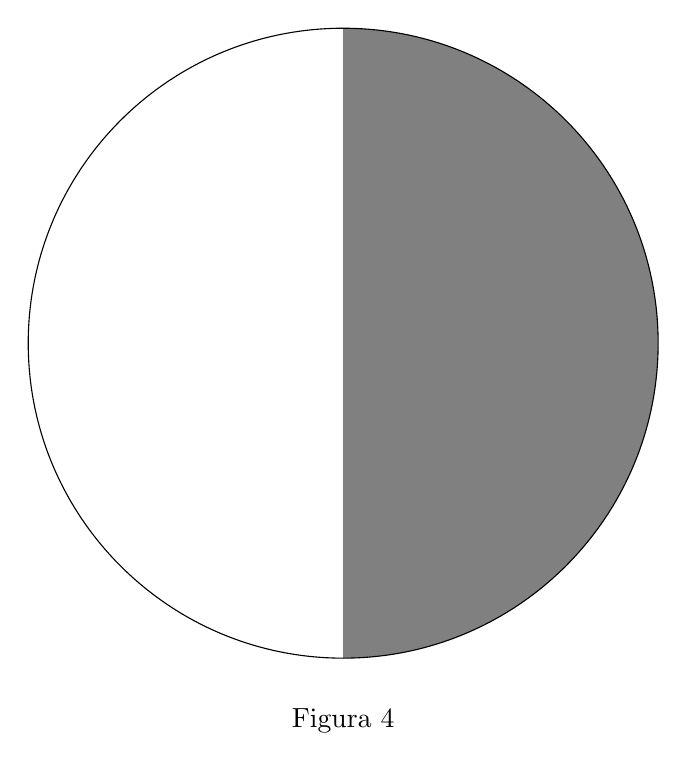
\begin{tikzpicture}[scale=2, x=1cm,y=1cm]
 \draw[fill=gray] (0,-2) arc (-90:90: 2);
 \draw (0,2) arc (90:270:2) (0,-2.4) node{Figura 4};
\end{tikzpicture}
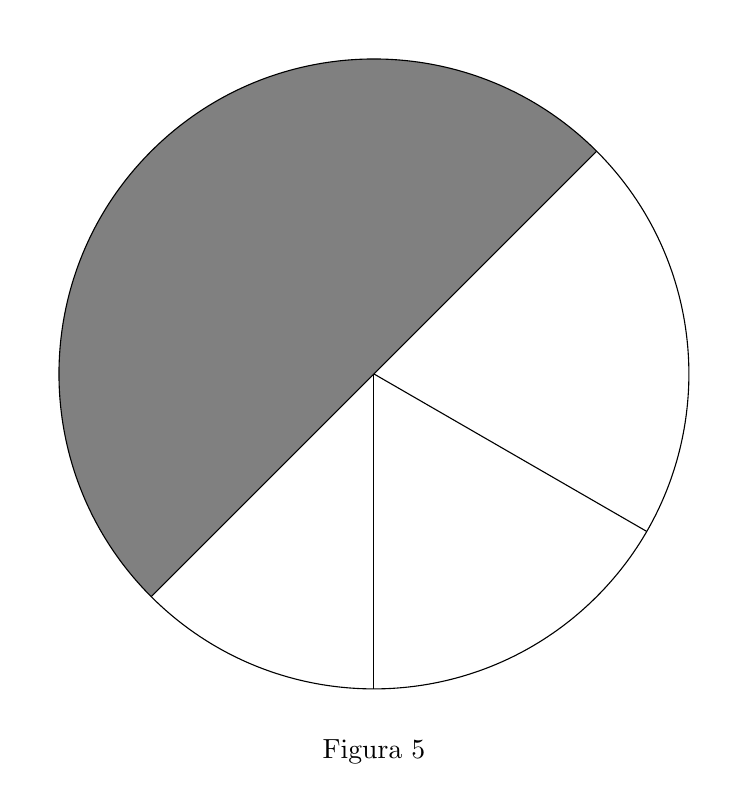
\begin{tikzpicture}[scale=2, x=1cm,y=1cm]
 \draw[fill=gray] (45:2) arc (45:225:2);
 \draw (225:2) arc (225:405:2) (0,-2.4) node{Figura 5};
 \draw (0,0) -- (0,-2);
 \draw (0,0) -- (-30:2);
 \draw (225:2) -- (45:2);
 \end{tikzpicture}

 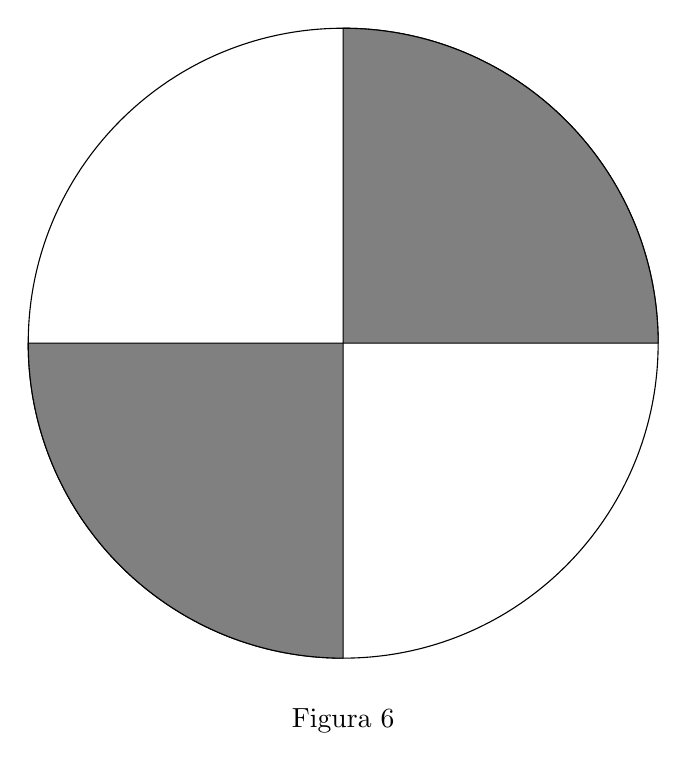
\begin{tikzpicture}[scale=2, x=1cm,y=1cm]
 \draw (0,0) circle (2);
 \draw[fill=gray] (0,0) -- (2,0) arc (0:90:2) -- cycle; 
 \draw[fill=gray] (0,0) -- (-2,0) arc (180:270: 2) -- cycle;
 \node at (0,-2.4) {Figura 6};
\end{tikzpicture}
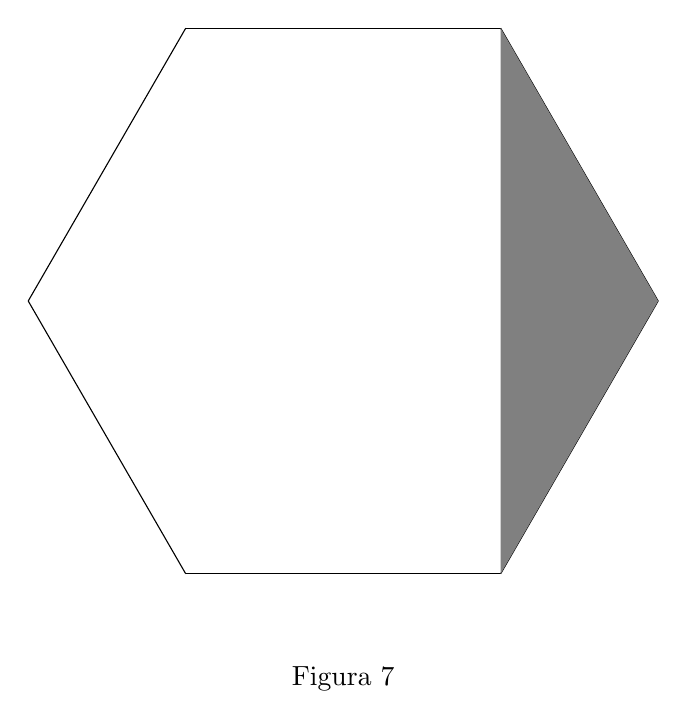
\begin{tikzpicture}[scale=2, x=1cm,y=1cm]% hexágonos
 \foreach \x in {0,60,...,300}{
 \draw (\x:2) -- (\x +60: 2);}
 \fill[gray] (2,0) -- (60:2) -- (300:2);
 \node at (0,-2.4) {Figura 7};
\end{tikzpicture}

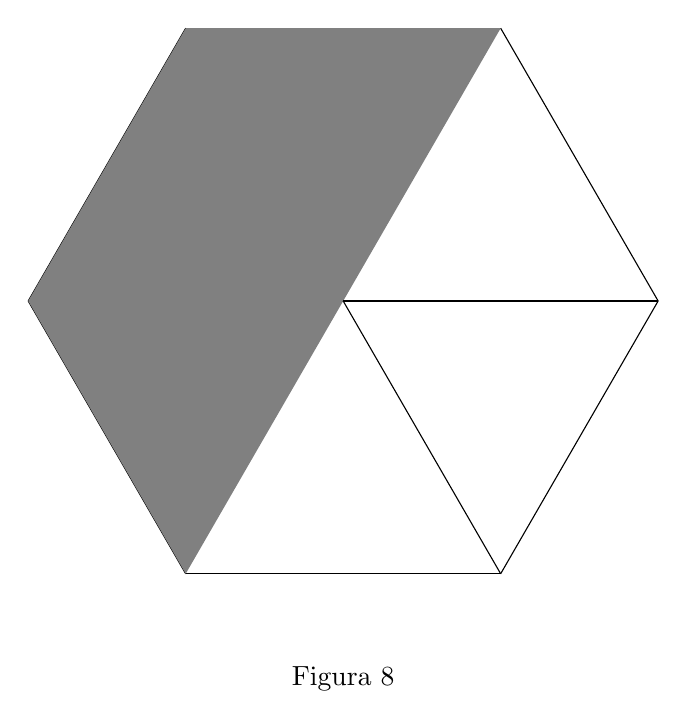
\begin{tikzpicture}[scale=2, x=1cm,y=1cm]
 \foreach \x in {0,60,...,300}{
 \draw (\x:2) -- (\x +60: 2);}
 \fill[gray] (60:2) -- (120:2) -- (180:2) -- (240:2) --cycle;
 \draw (0,0) -- (2,0);
 \draw (0,0) -- (300:2) (0,-2.4) node{Figura 8};
\end{tikzpicture}
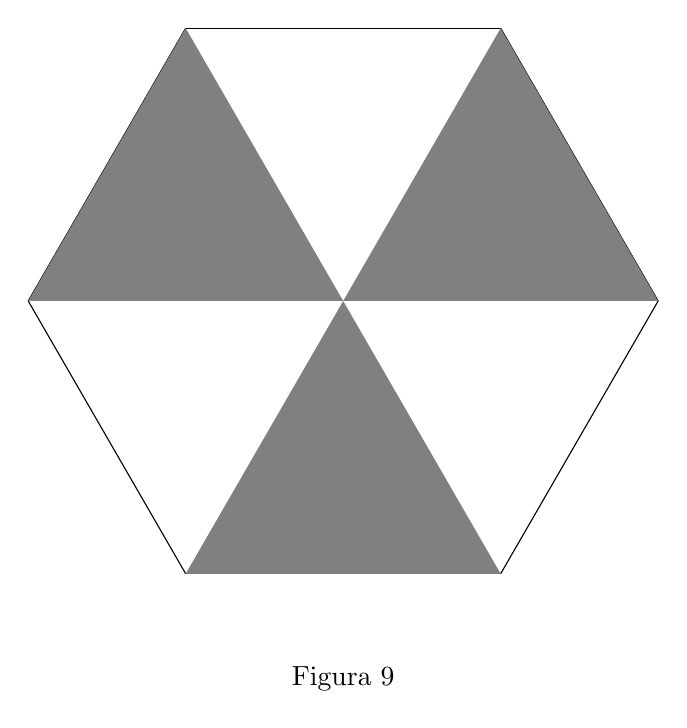
\begin{tikzpicture}[scale=2, x=1cm,y=1cm]
 \foreach \x in {0,60,...,300}{
 \draw (\x:2) -- (\x +60: 2);}
 \fill[gray] (0:2) -- (60:2) -- (0:0) --cycle;
 \fill[gray] (120:2) -- (180:2) -- (0:0) --cycle;
 \fill[gray] (240:2) -- (300:2) -- (0:0) --cycle;
 \node at (0,-2.4) {Figura 9};
\end{tikzpicture}

%círculo

\noindent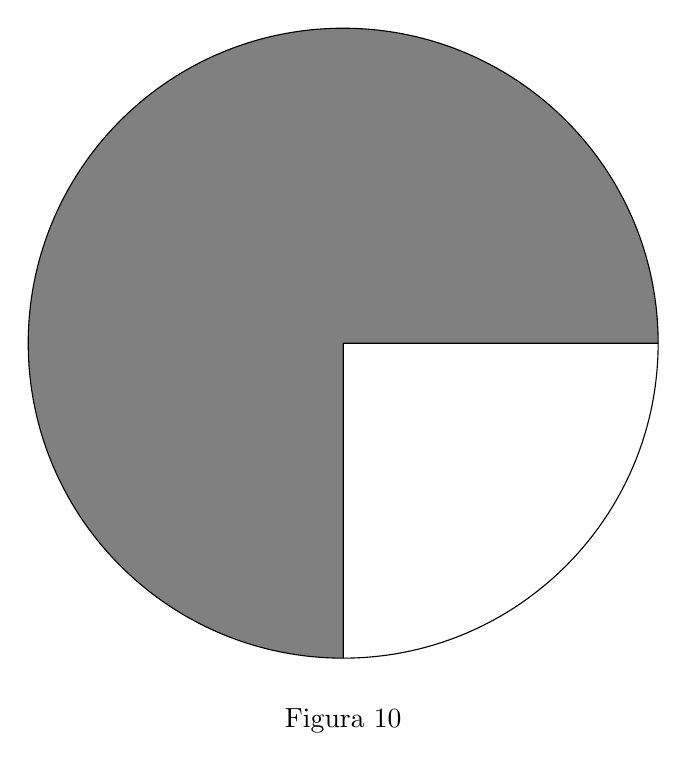
\begin{tikzpicture}[scale=2, x=1cm,y=1cm]
 \draw[fill=gray] (0:2) arc (0:270:2) -- (0,0) -- cycle;
 \draw (270:2) arc (270:360:2);
 \draw (0,0) -- (0,-2);
 \draw (0,0) -- (2,0)  (0,-2.4) node{Figura 10};
 \end{tikzpicture}
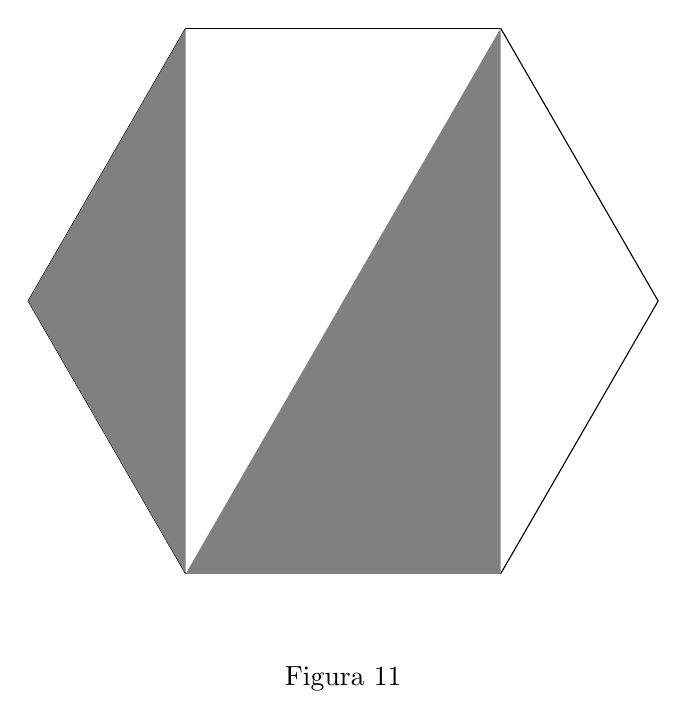
\begin{tikzpicture}[scale=2, x=1cm,y=1cm]%hexágonos
 \foreach \x in {0,60,...,300}{
 \draw (\x:2) -- (\x +60: 2);}
\fill[gray] (120:2) -- (180:2) -- (240:2) -- cycle;
\fill[gray] (240:2) -- (300:2) -- (60:2) -- cycle;
 \node at (0,-2.4) {Figura 11};
\end{tikzpicture}

%retângulo
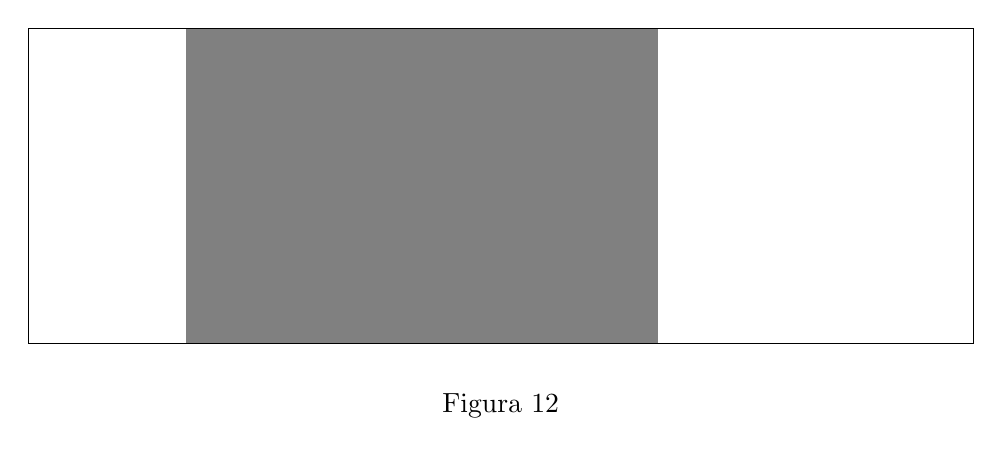
\begin{tikzpicture}[scale=2, x=1cm,y=1cm]
 \fill[gray] (1,0) rectangle (4,2);
 \draw (0,0) rectangle (6,2);
 \node at (3,-0.4) {Figura 12};
 \end{tikzpicture}


\noindent{\bf Atividade 10}
  \vspace{.2cm}
  
 \begin{longtable}{cc}
 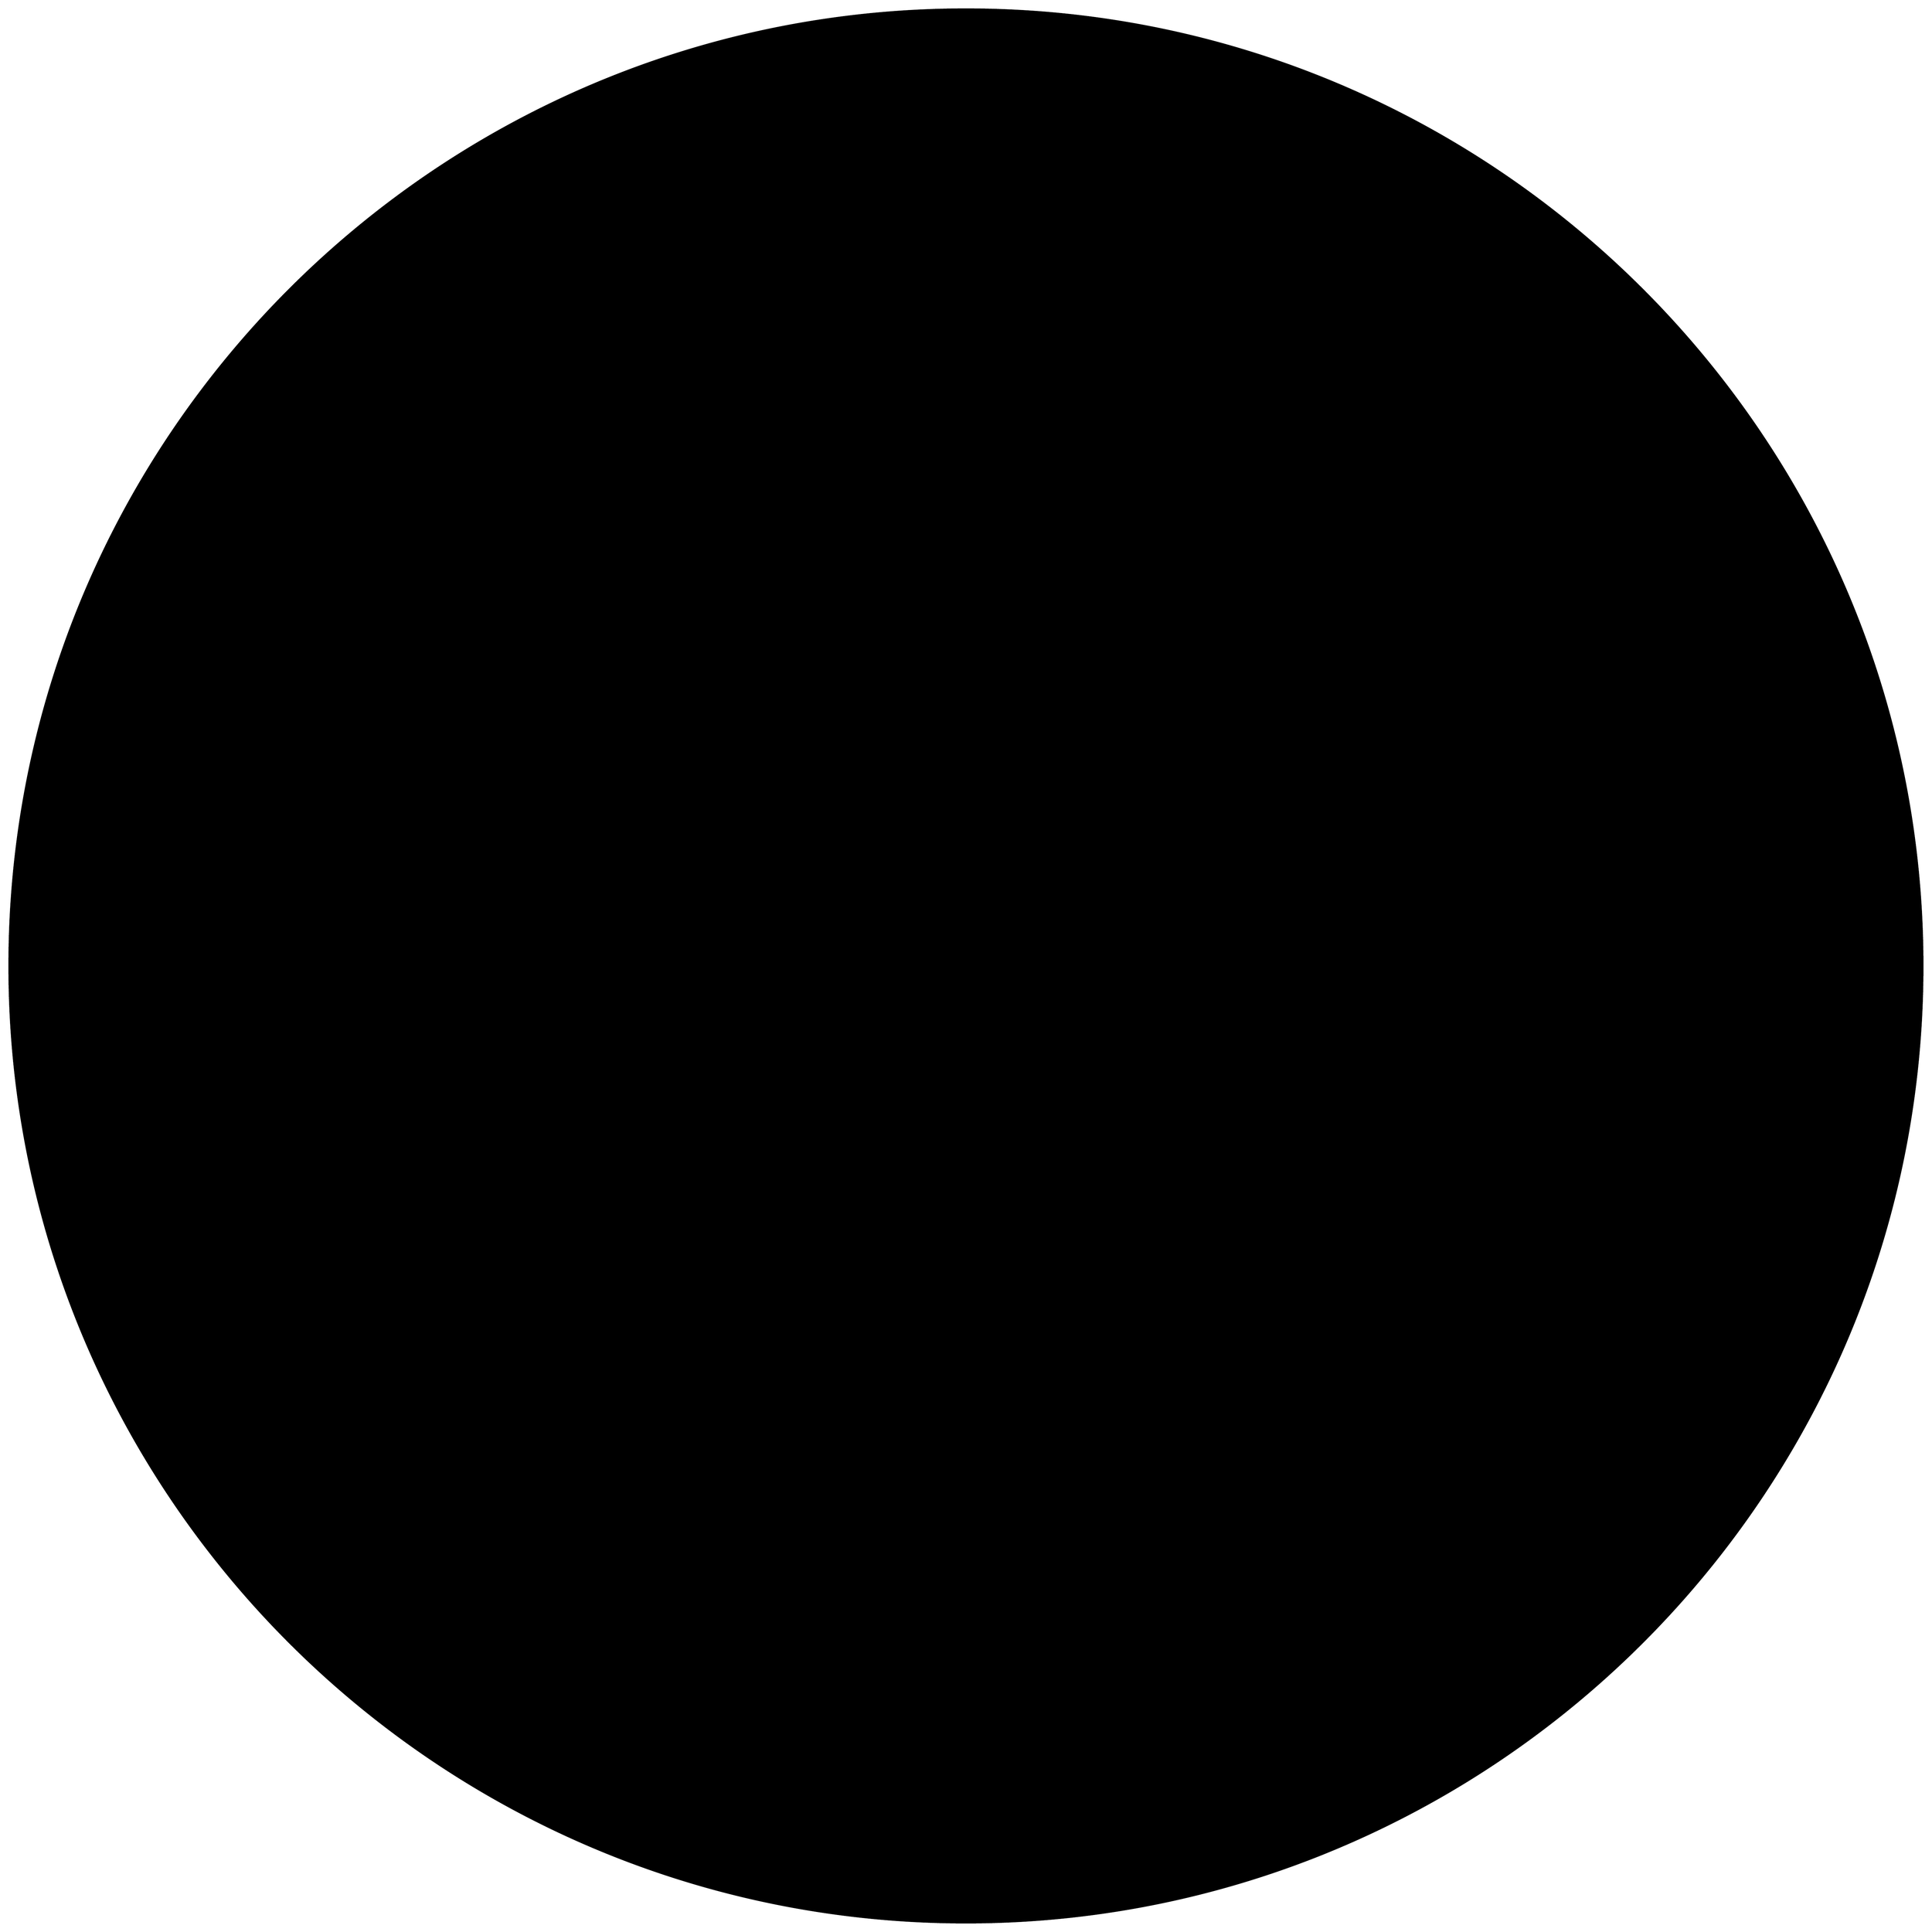
\begin{tikzpicture}
\fill[black] (0,0) circle (40);
 \end{tikzpicture}
&
 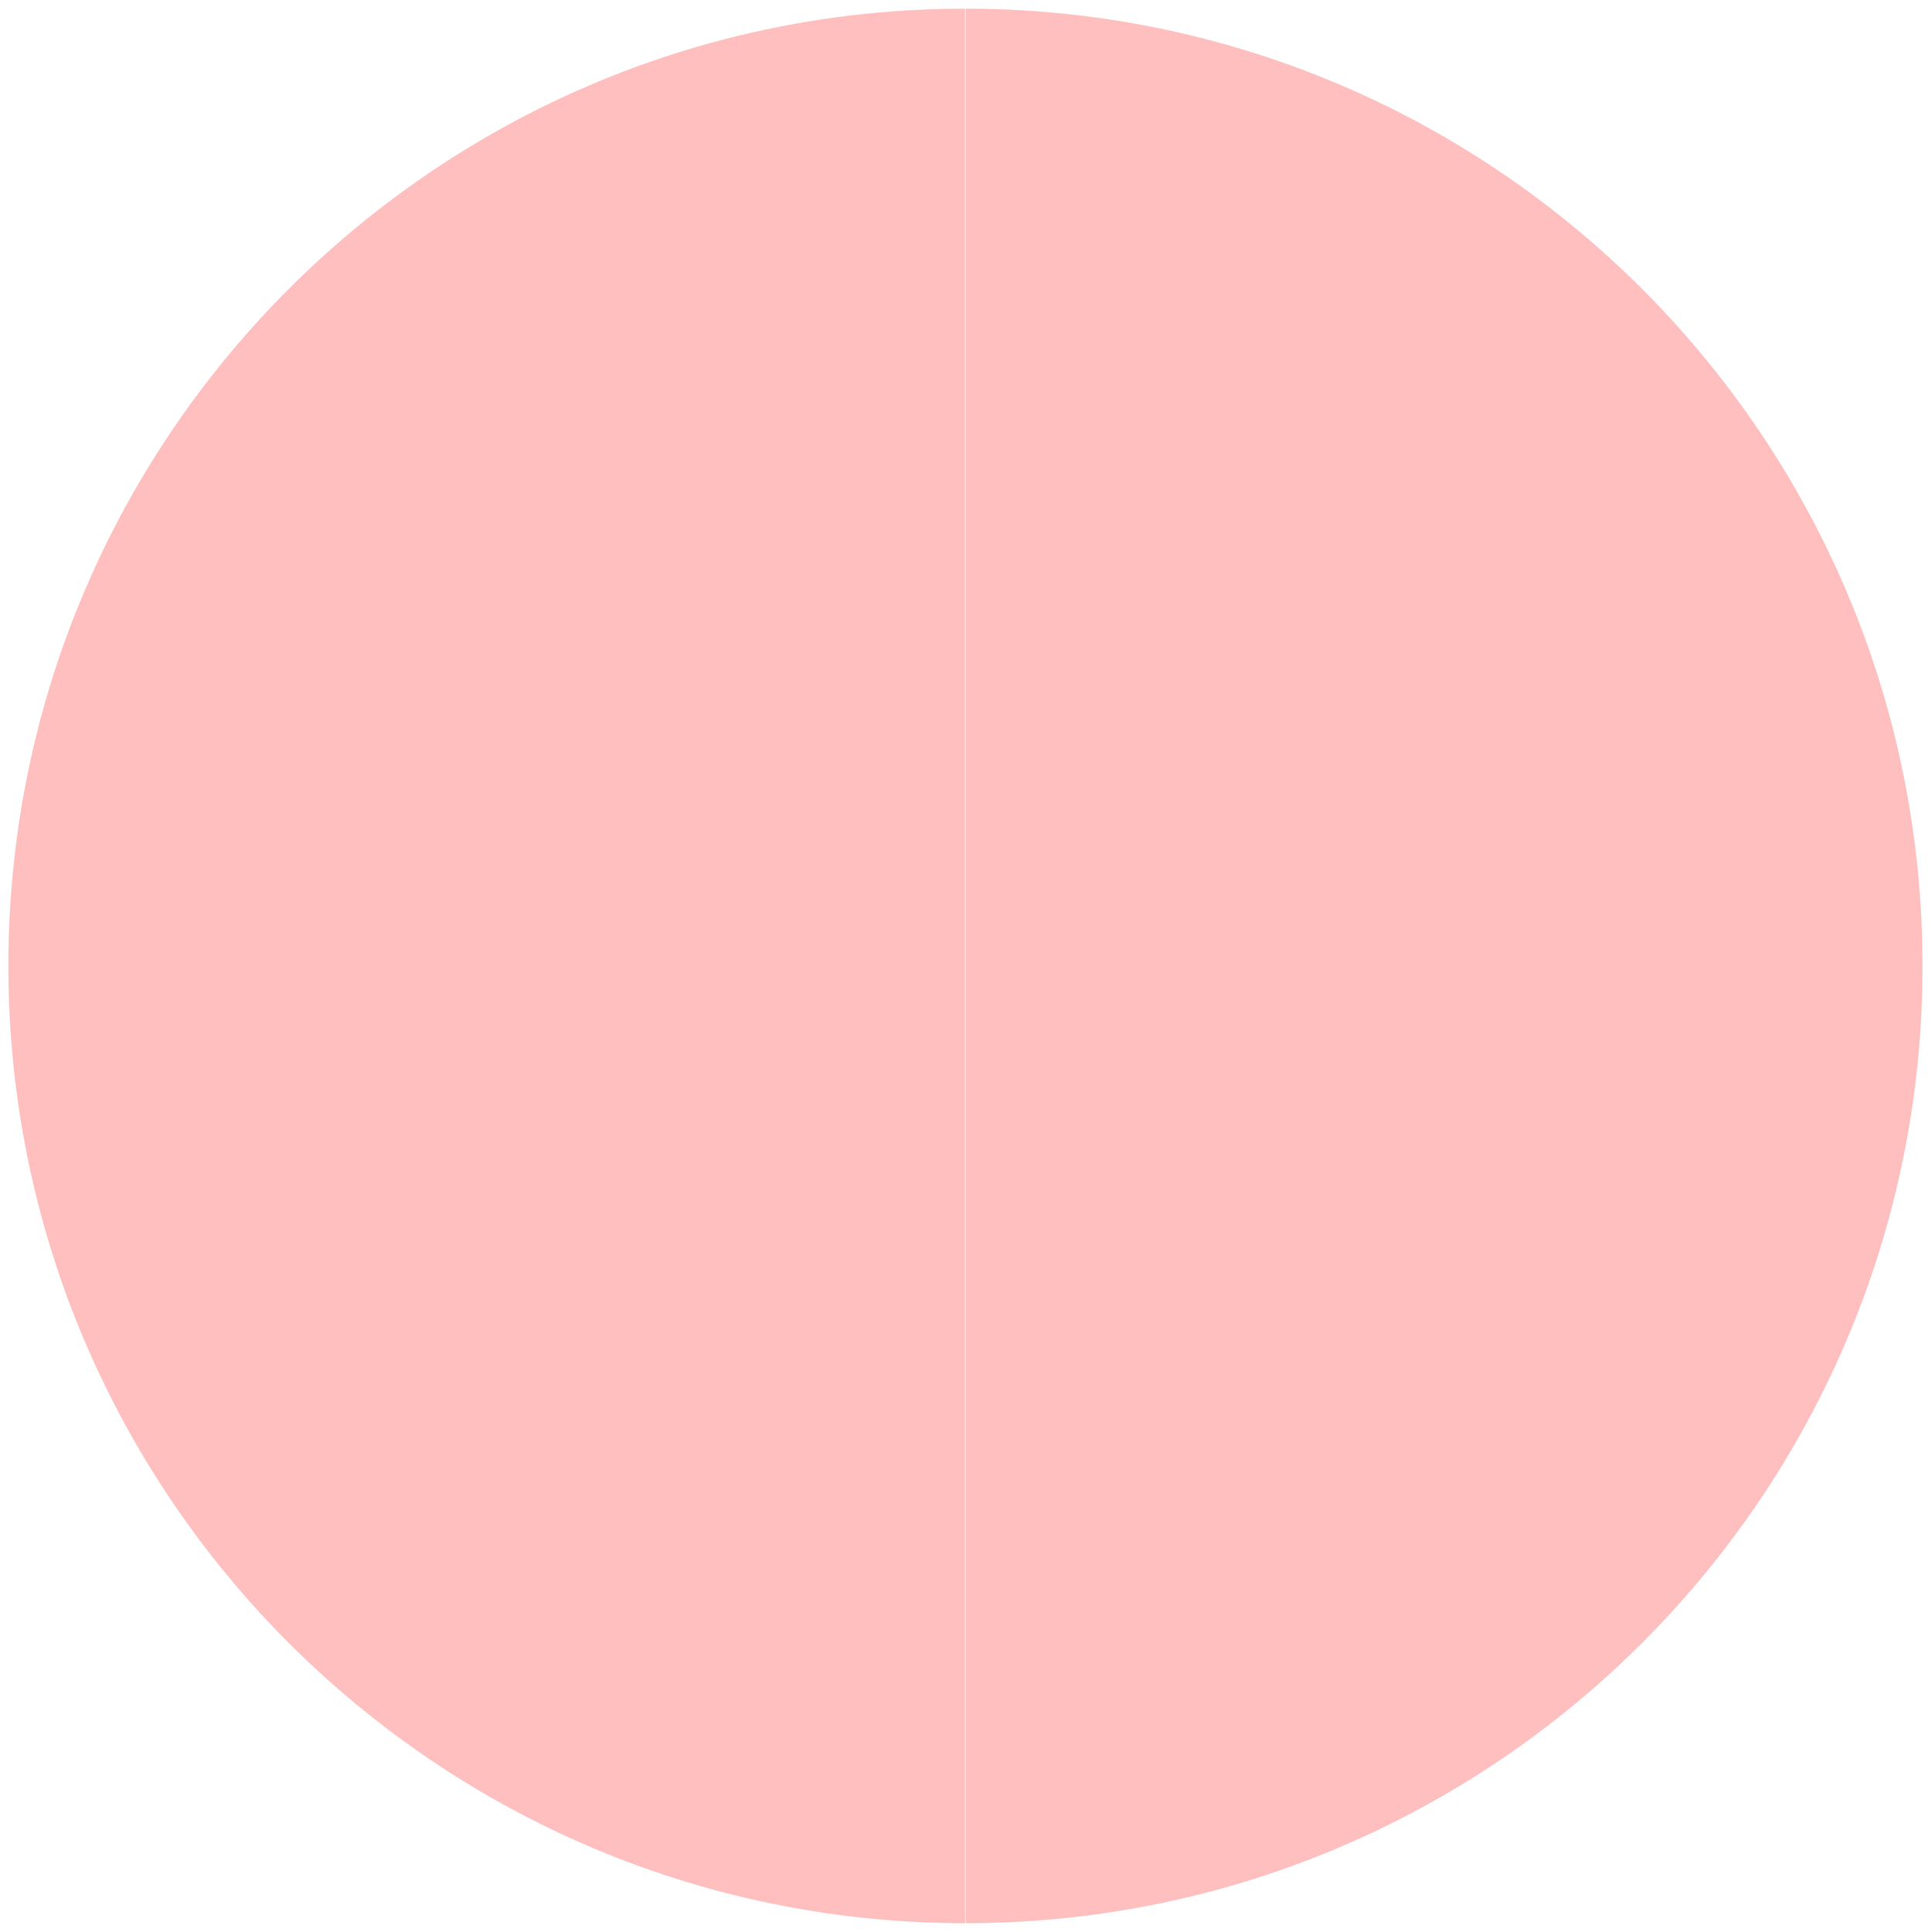
\begin{tikzpicture}
\fill[pink] (0,0) circle (40);
\draw[line width =.25mm, white] (-90:40) -- (90:40);	
\end{tikzpicture}
\\
 \begin{tikzpicture}
\fill[common] (0,0) circle (40);
\foreach \x in {30,150,270} \draw[line width =.25mm, white] (0,0)--(\x:40);
\end{tikzpicture}
&
 \begin{tikzpicture}
\fill[attention] (0,0) circle (40);
\foreach \x in {0,90} \draw[line width =.25mm, white] (\x:-40)--(\x:40);
\end{tikzpicture}
\\
 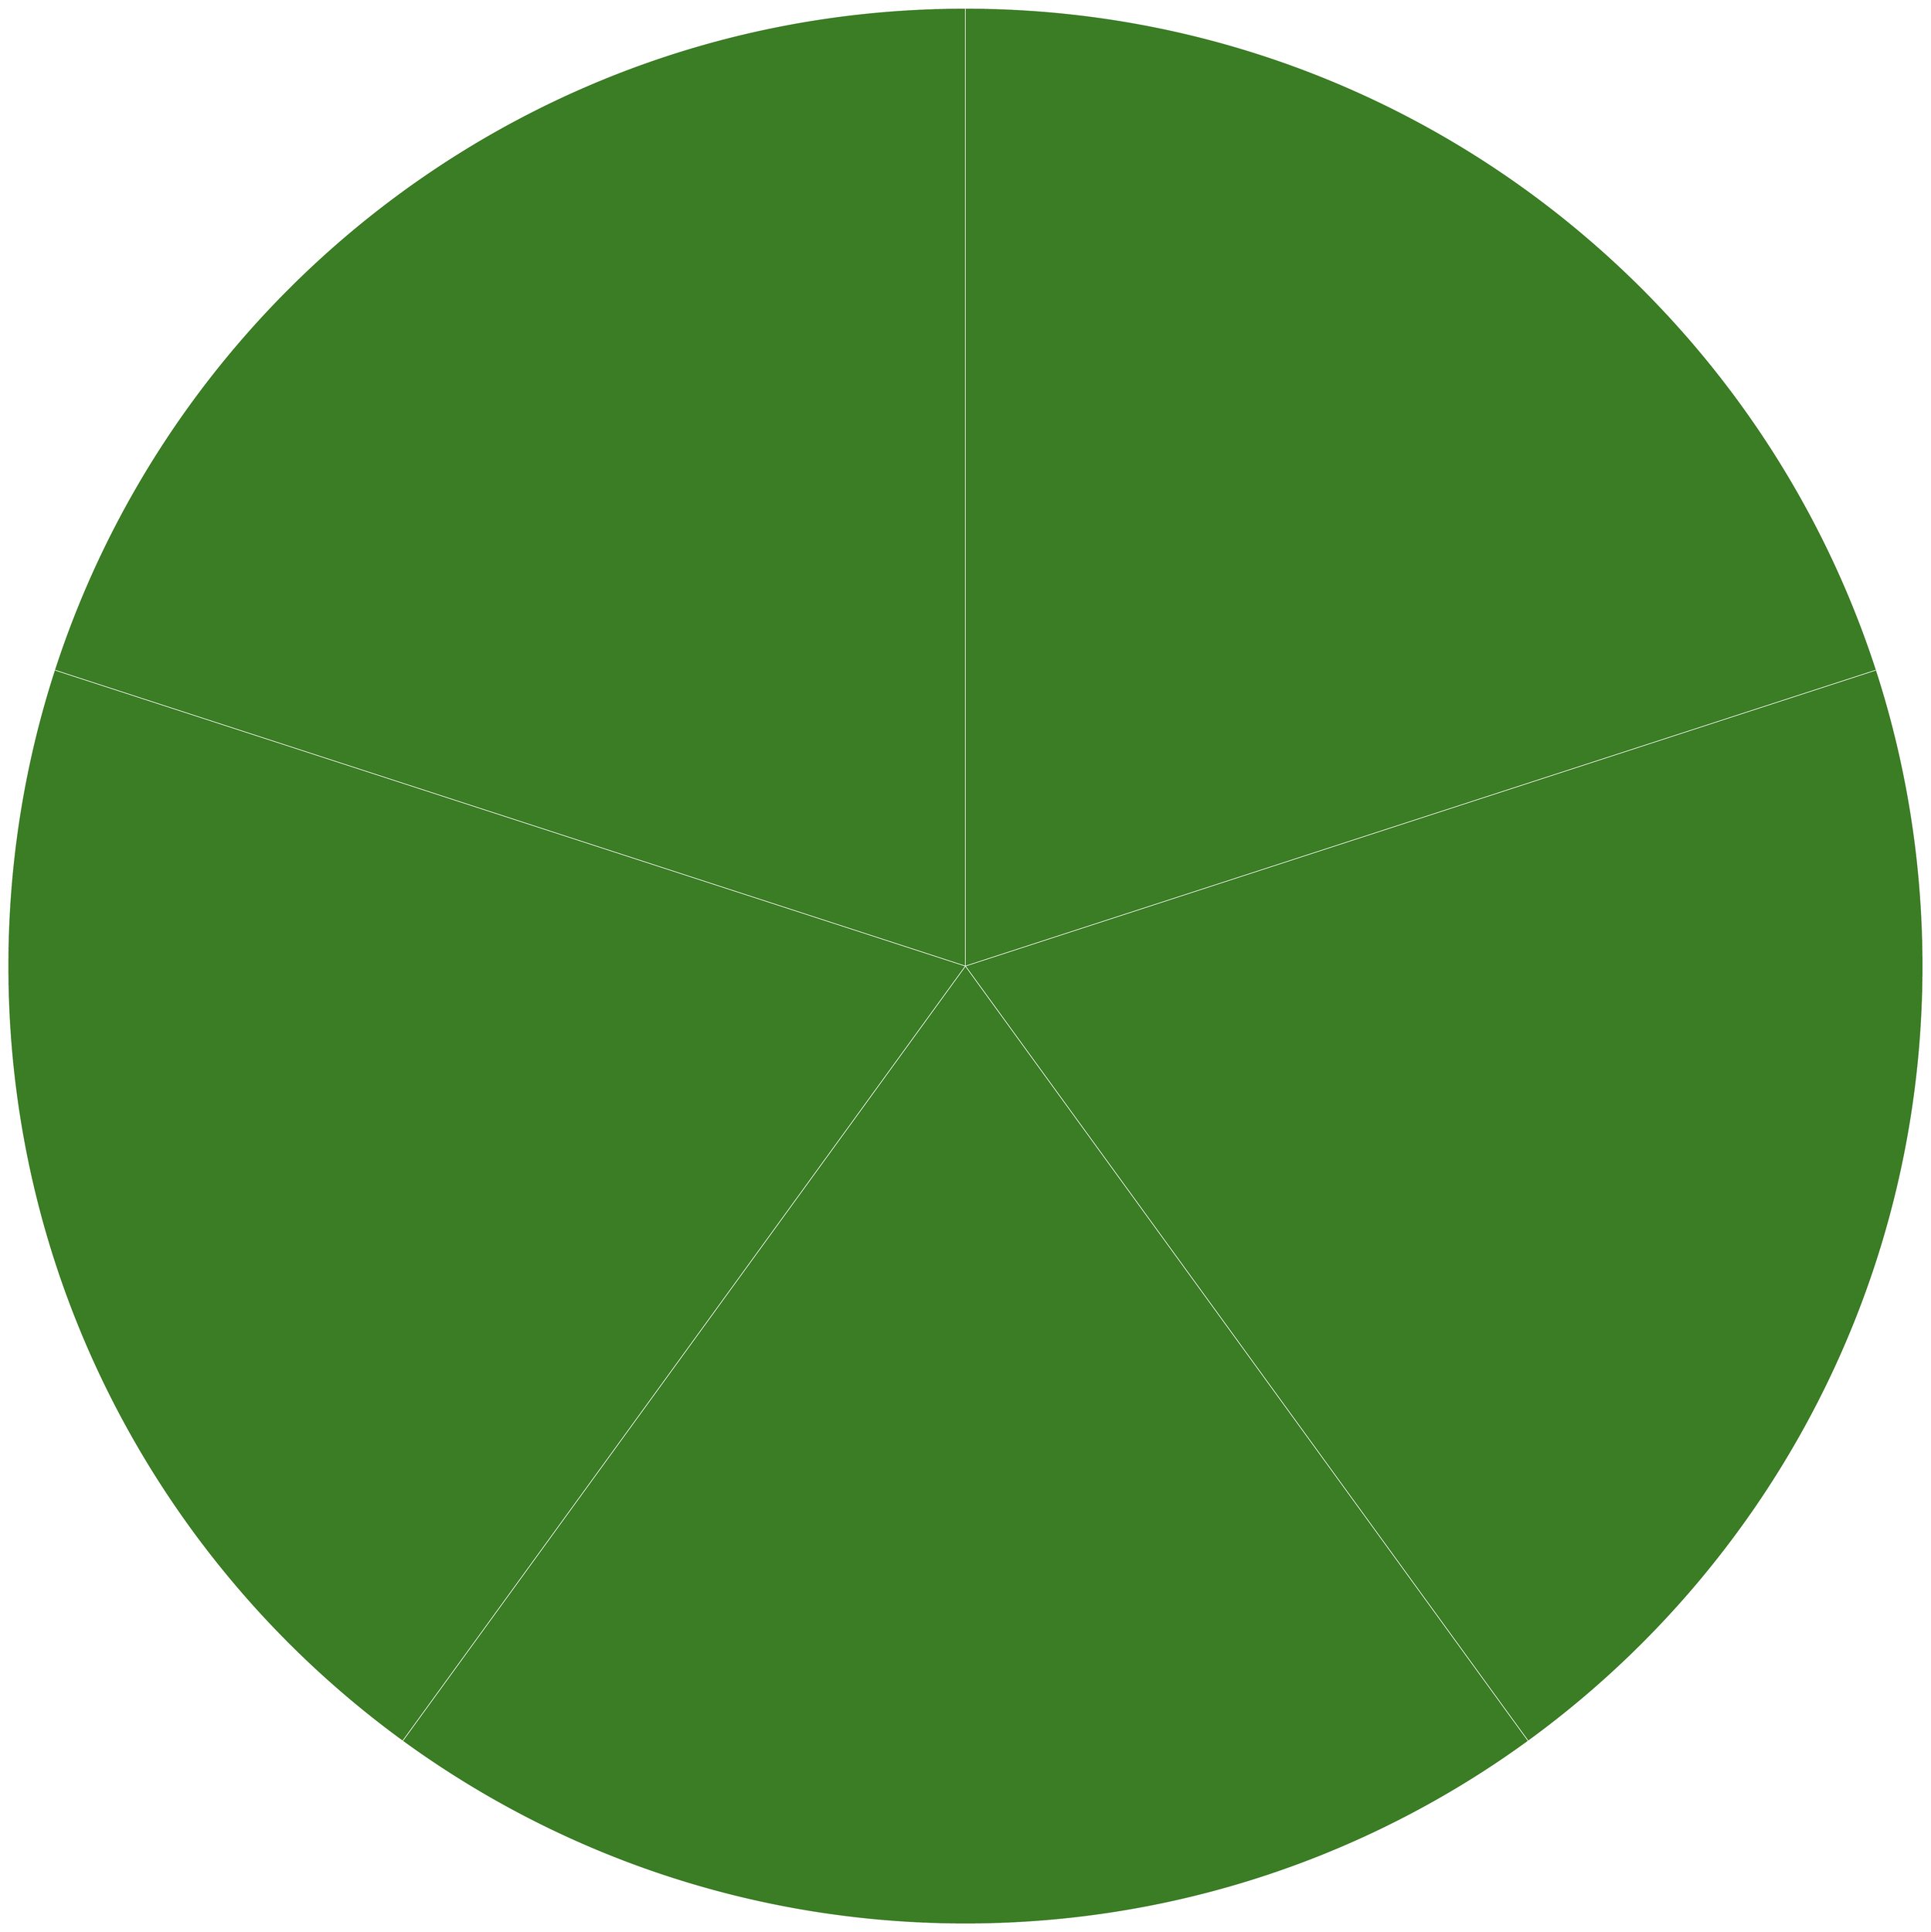
\begin{tikzpicture}
\fill[OliveGreen] (0,0) circle (40);
\foreach \x in {18,90,...,360} \draw[line width =.25mm, white] (0,0)--(\x:40);
\end{tikzpicture}
&
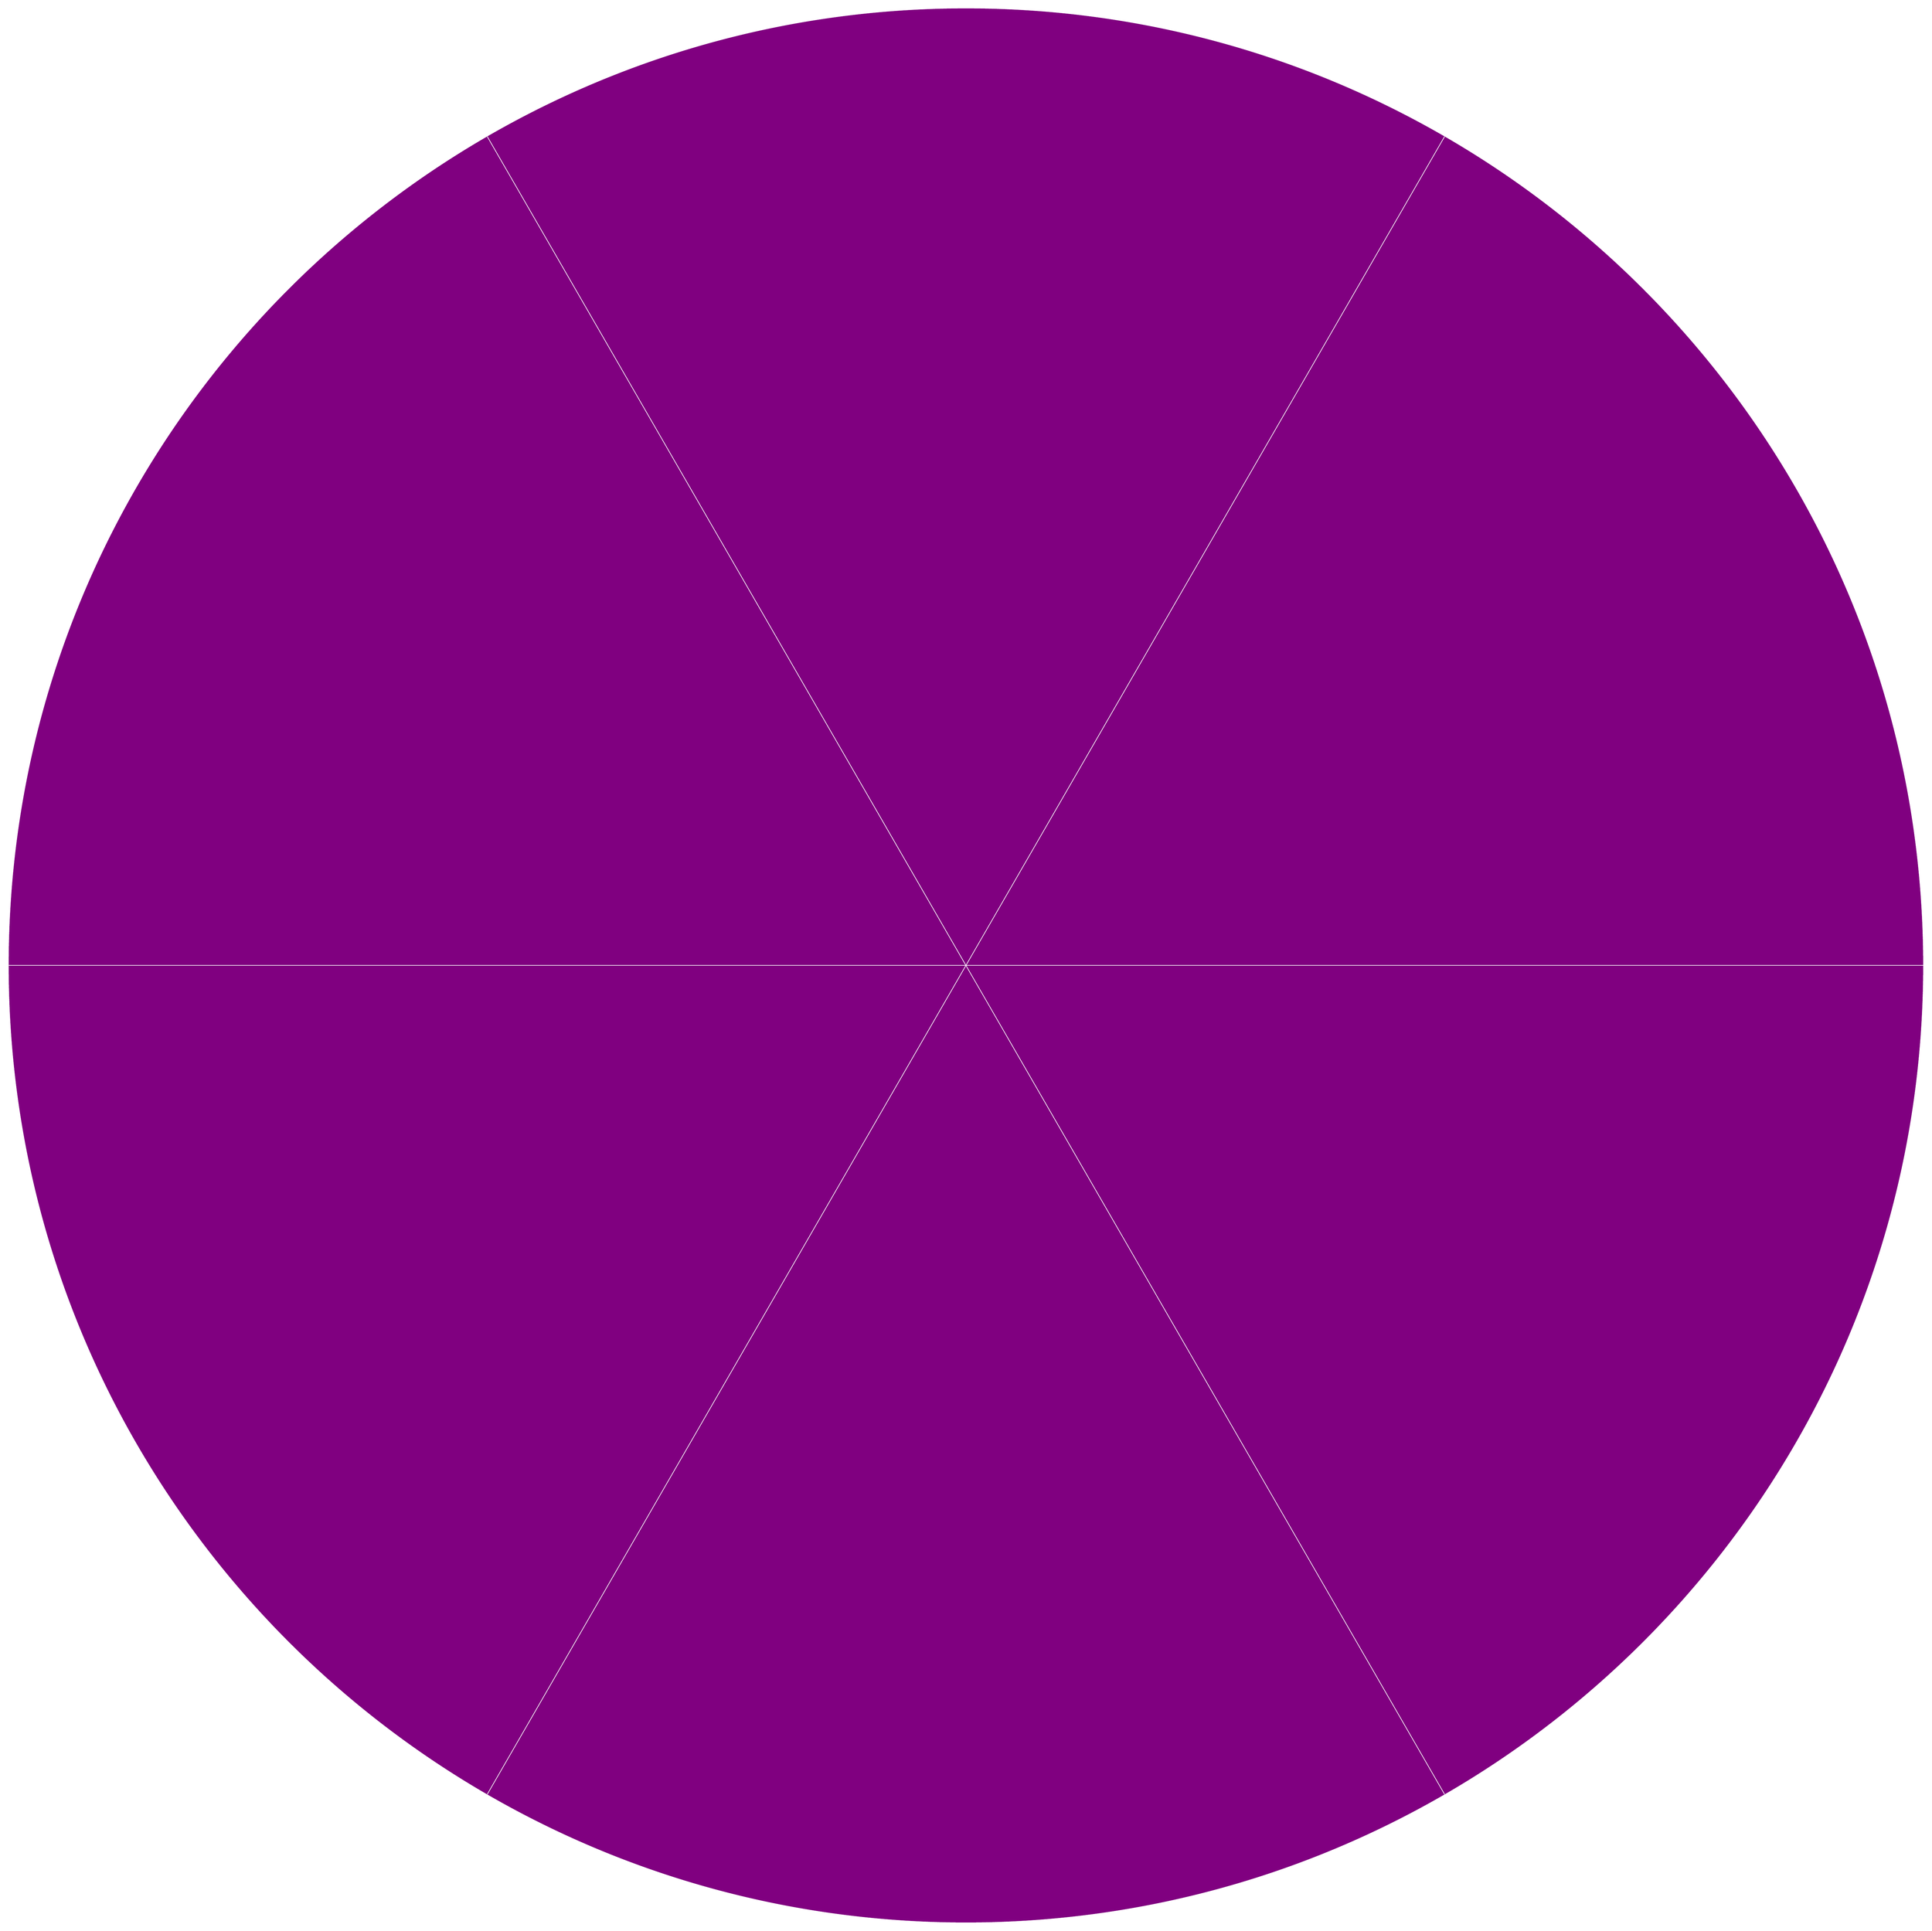
\begin{tikzpicture}
\fill[Purple] (0,0) circle (40);
\foreach \x in {0,60,...,360} \draw[line width =.25mm, white] (0,0)--(\x:40);
\end{tikzpicture}
\\
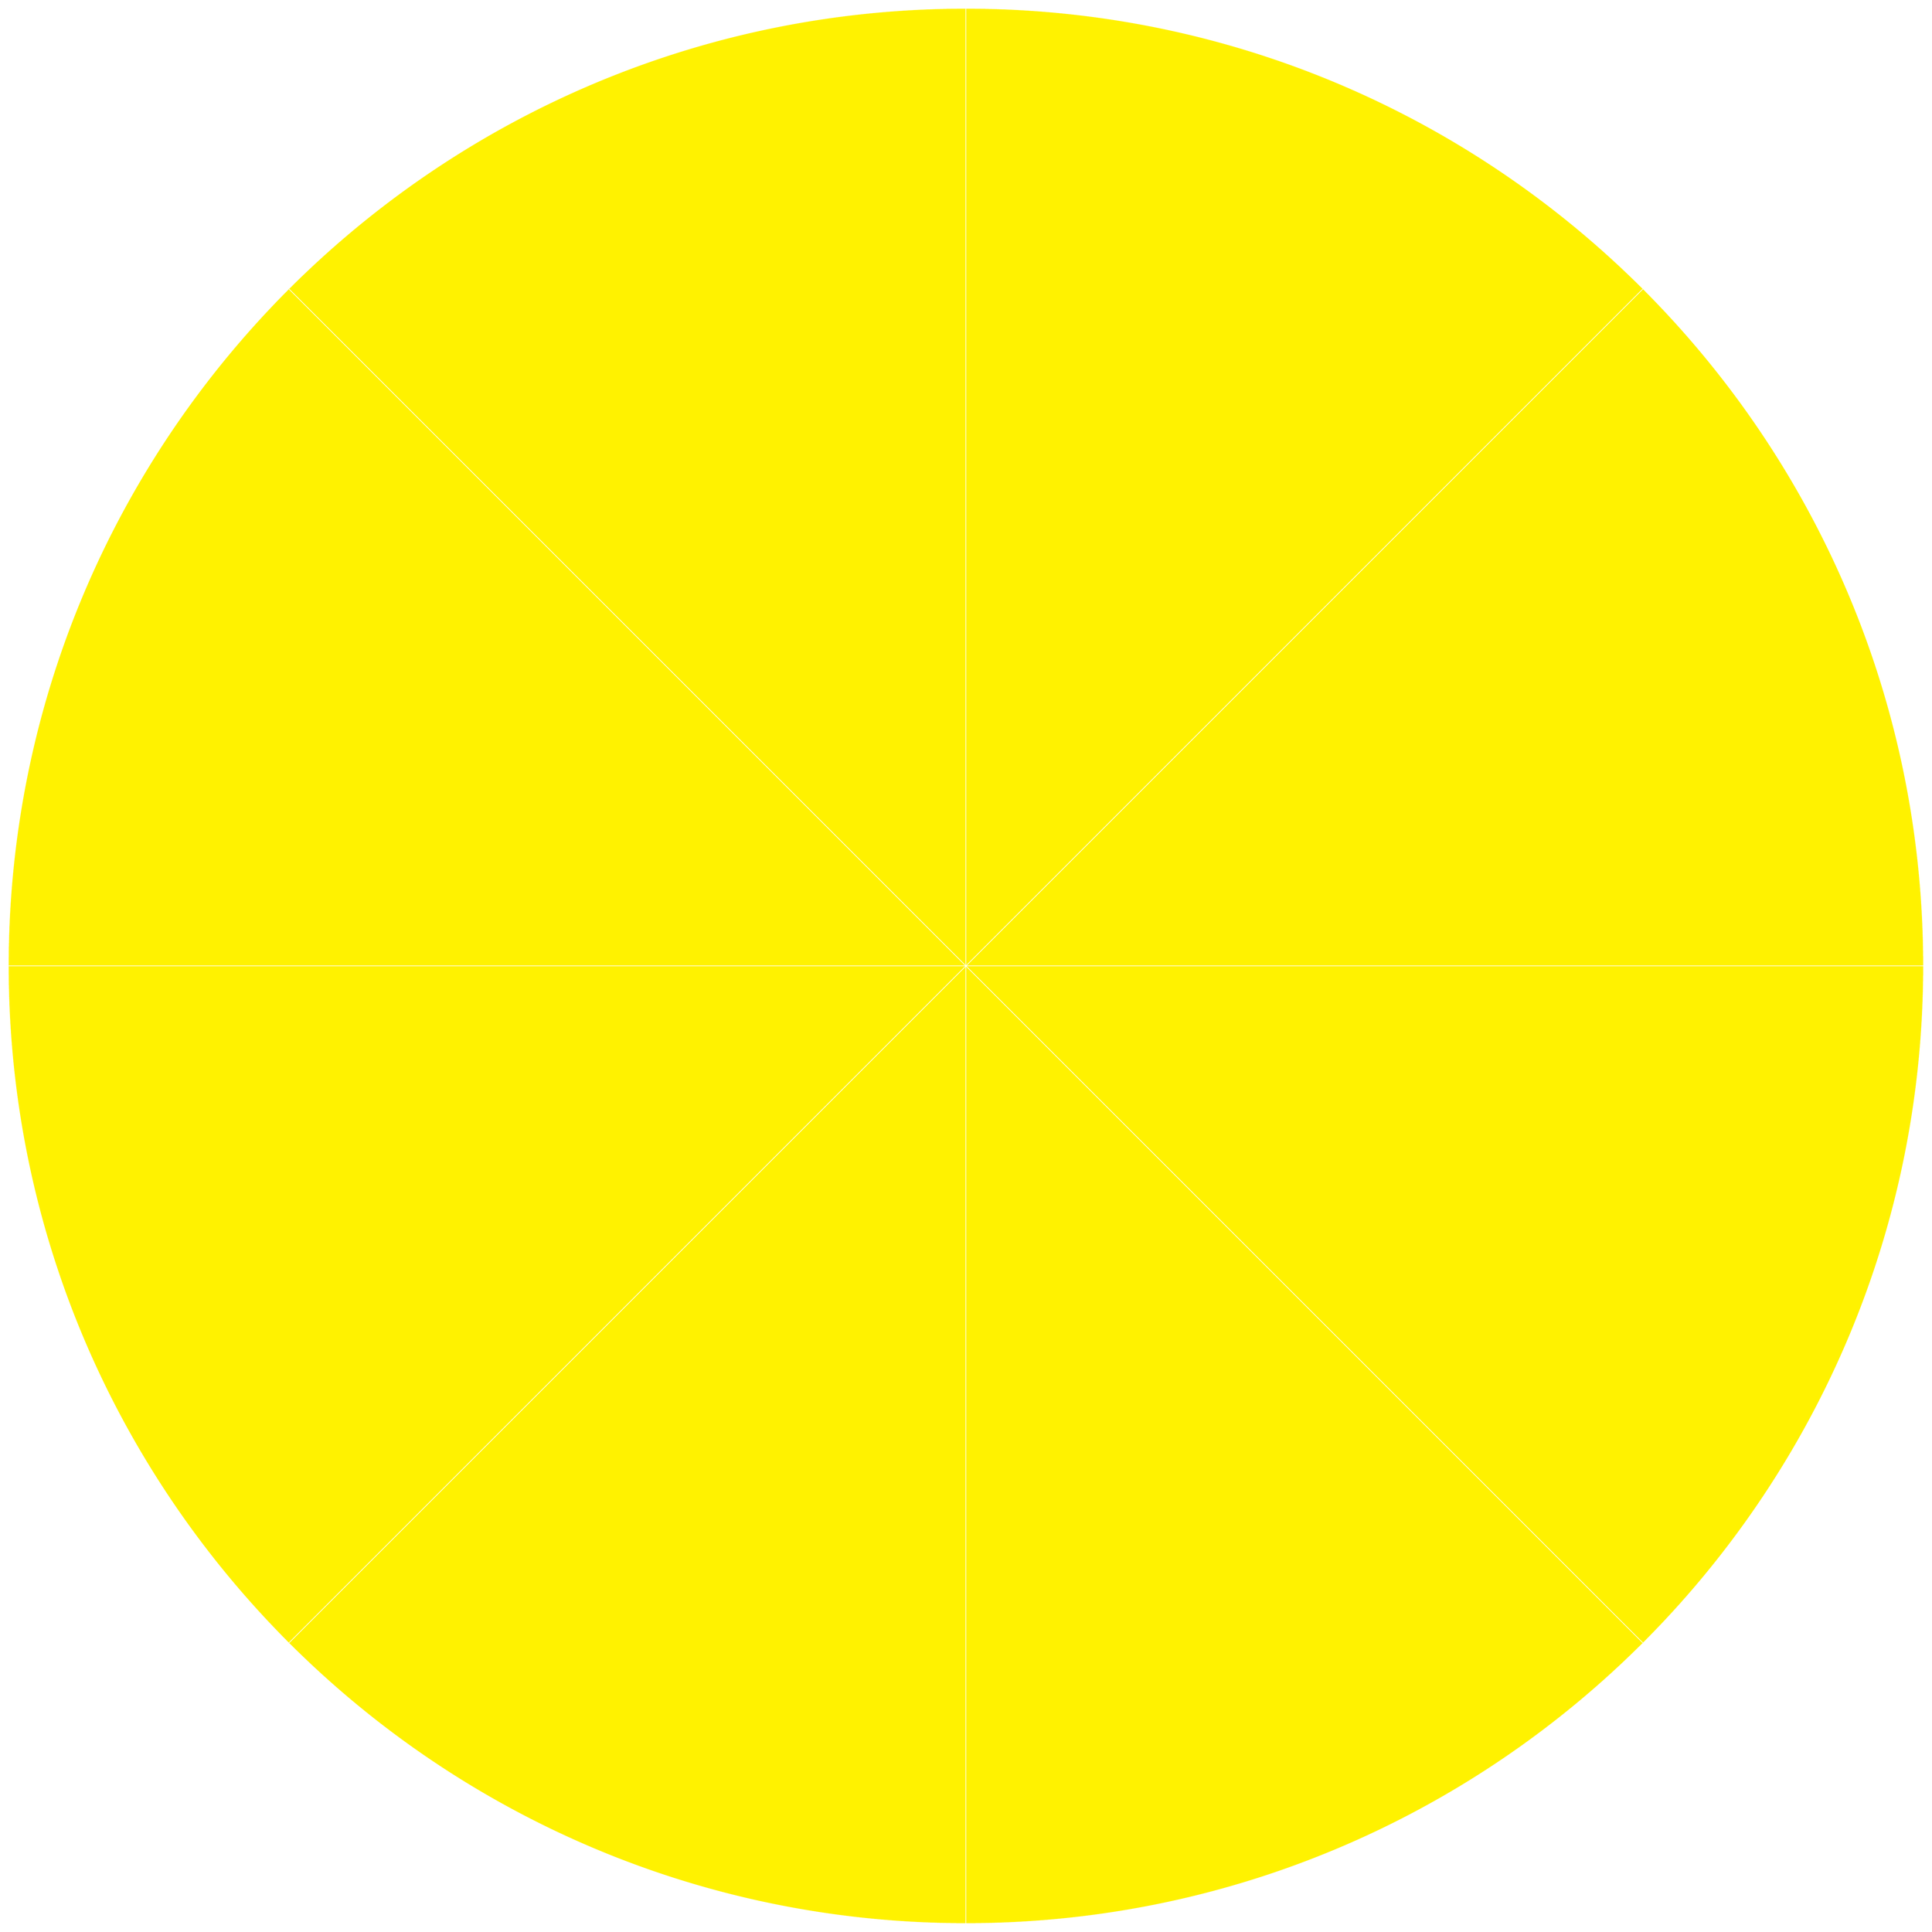
\begin{tikzpicture}
\fill[yellow] (0,0) circle (40);
\foreach \x in {0,45,...,360} \draw[line width =.25mm, white] (0,0)--(\x:40);
\end{tikzpicture}
&
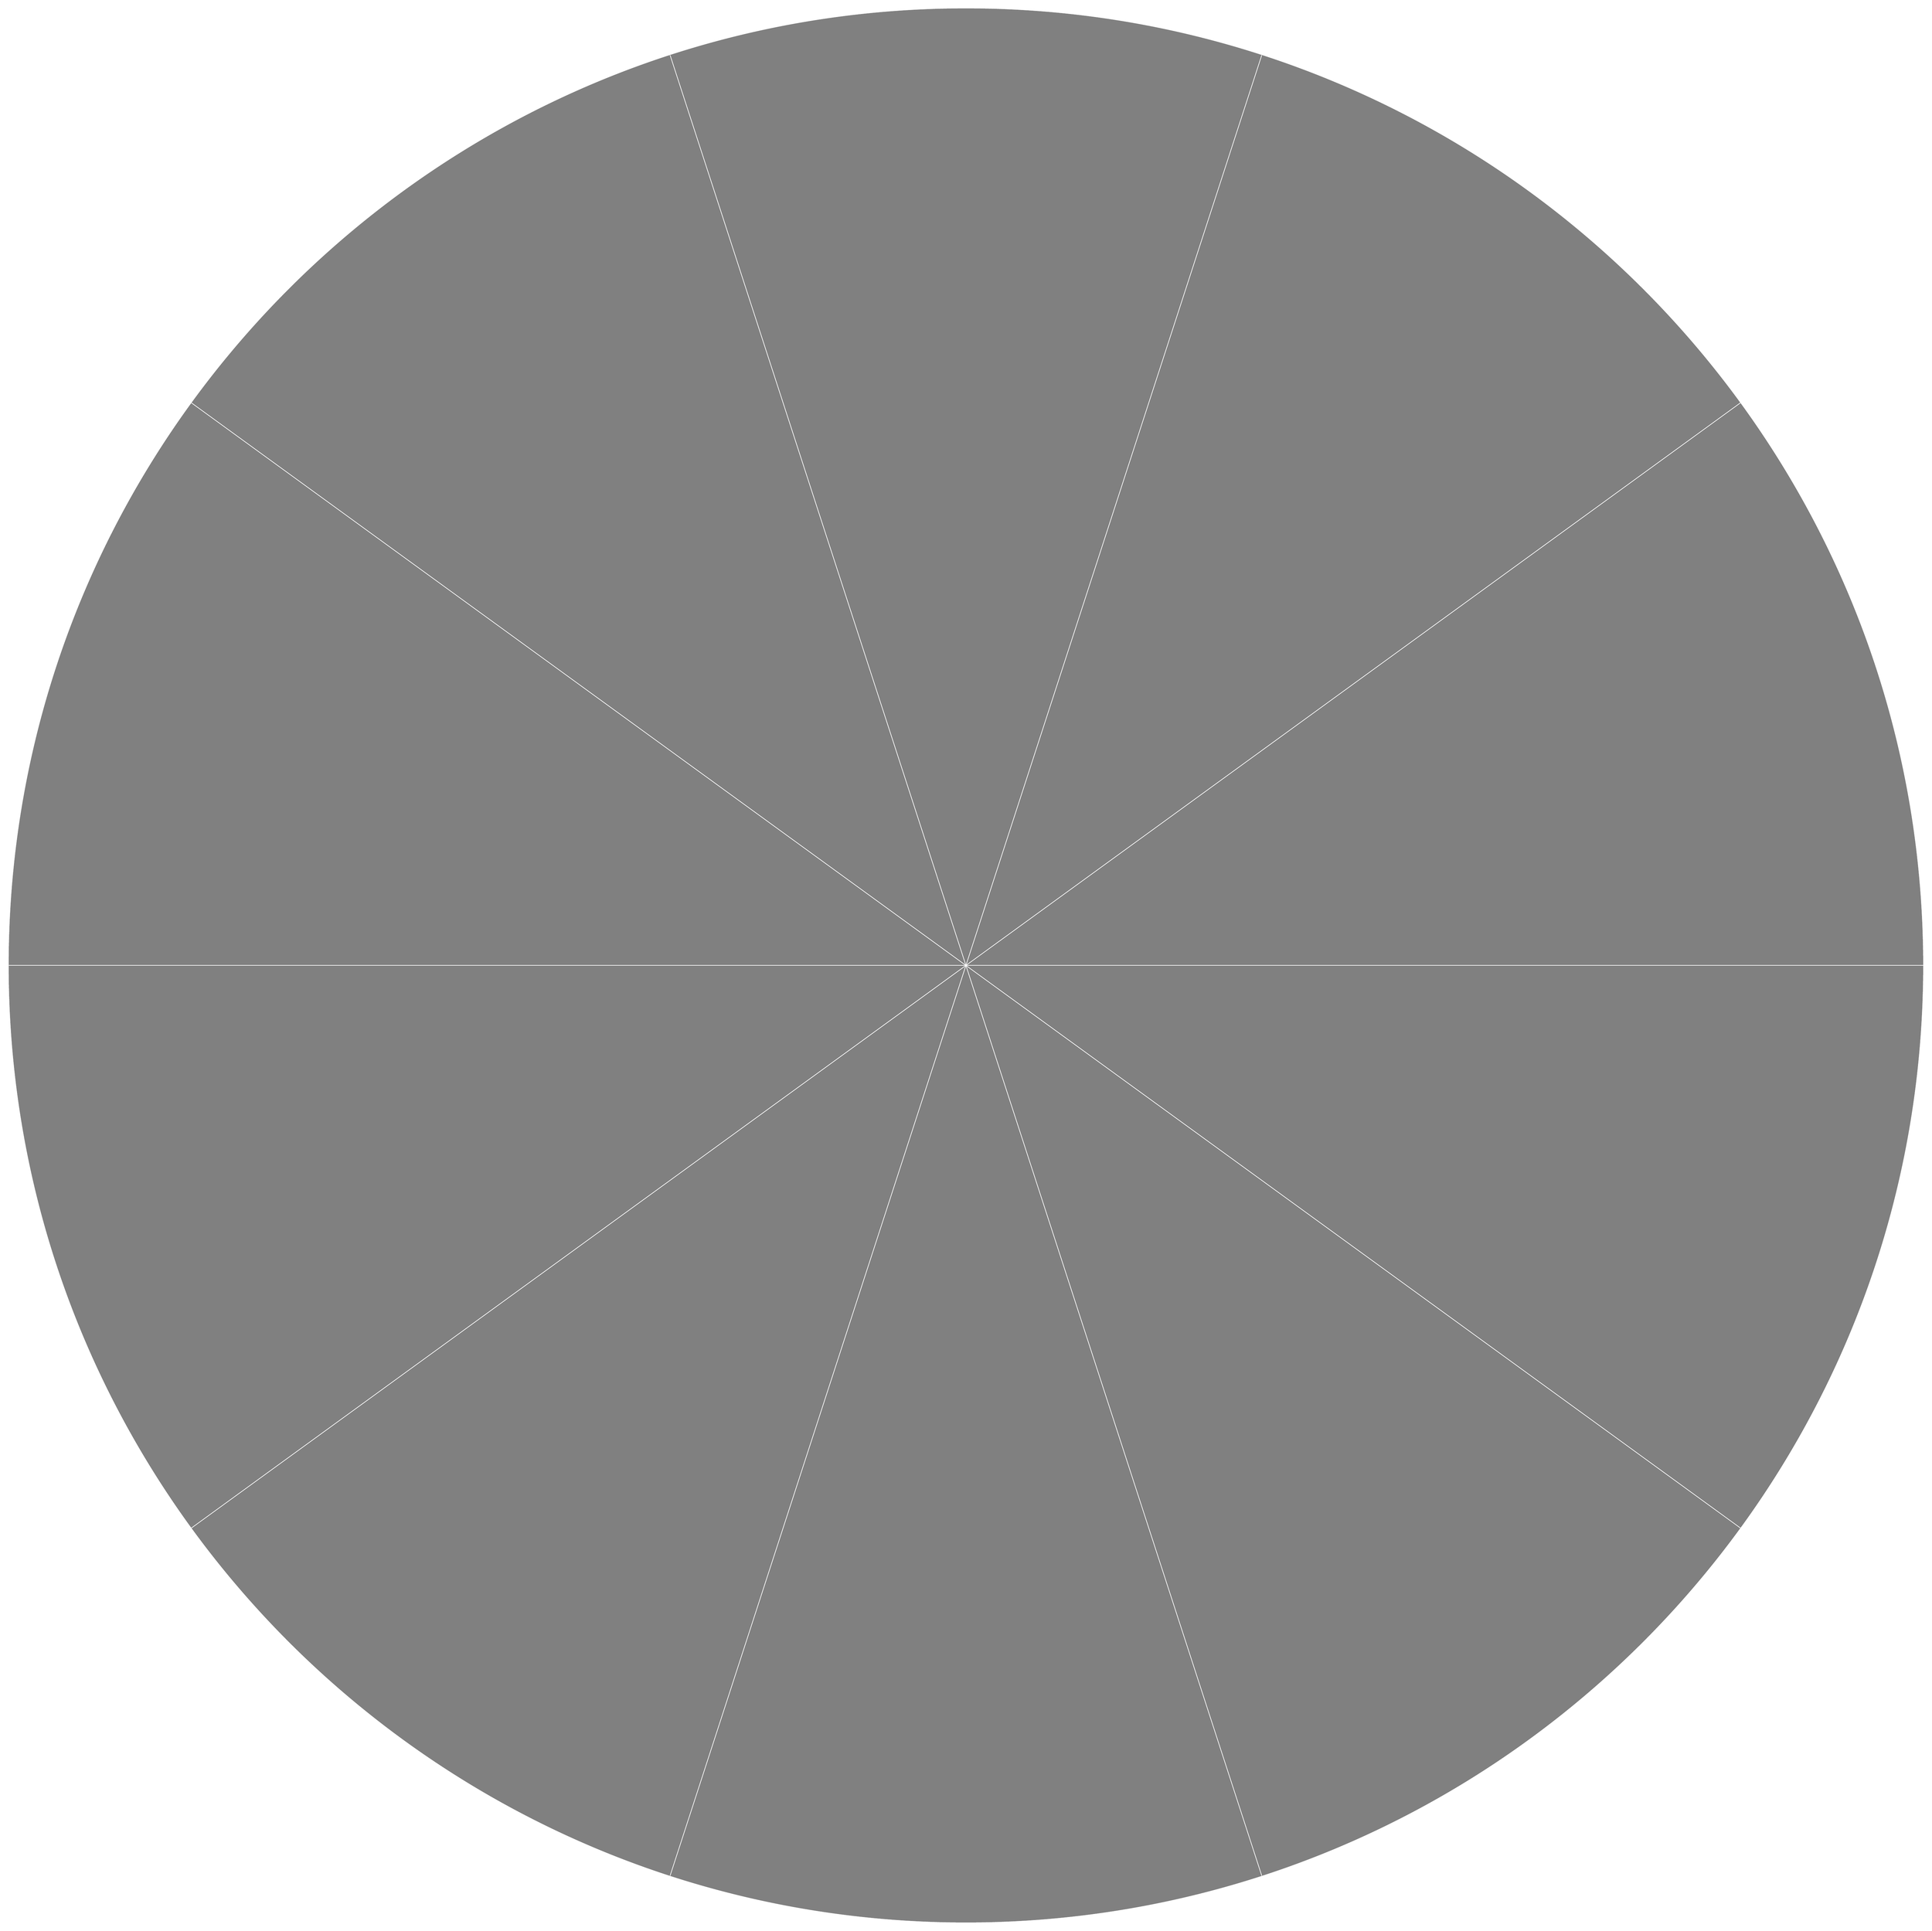
\begin{tikzpicture}
\fill[gray] (0,0) circle (40);
\foreach \x in {0,36,...,360} \draw[line width =.25mm, white] (0,0)--(\x:40);
\end{tikzpicture}
\\
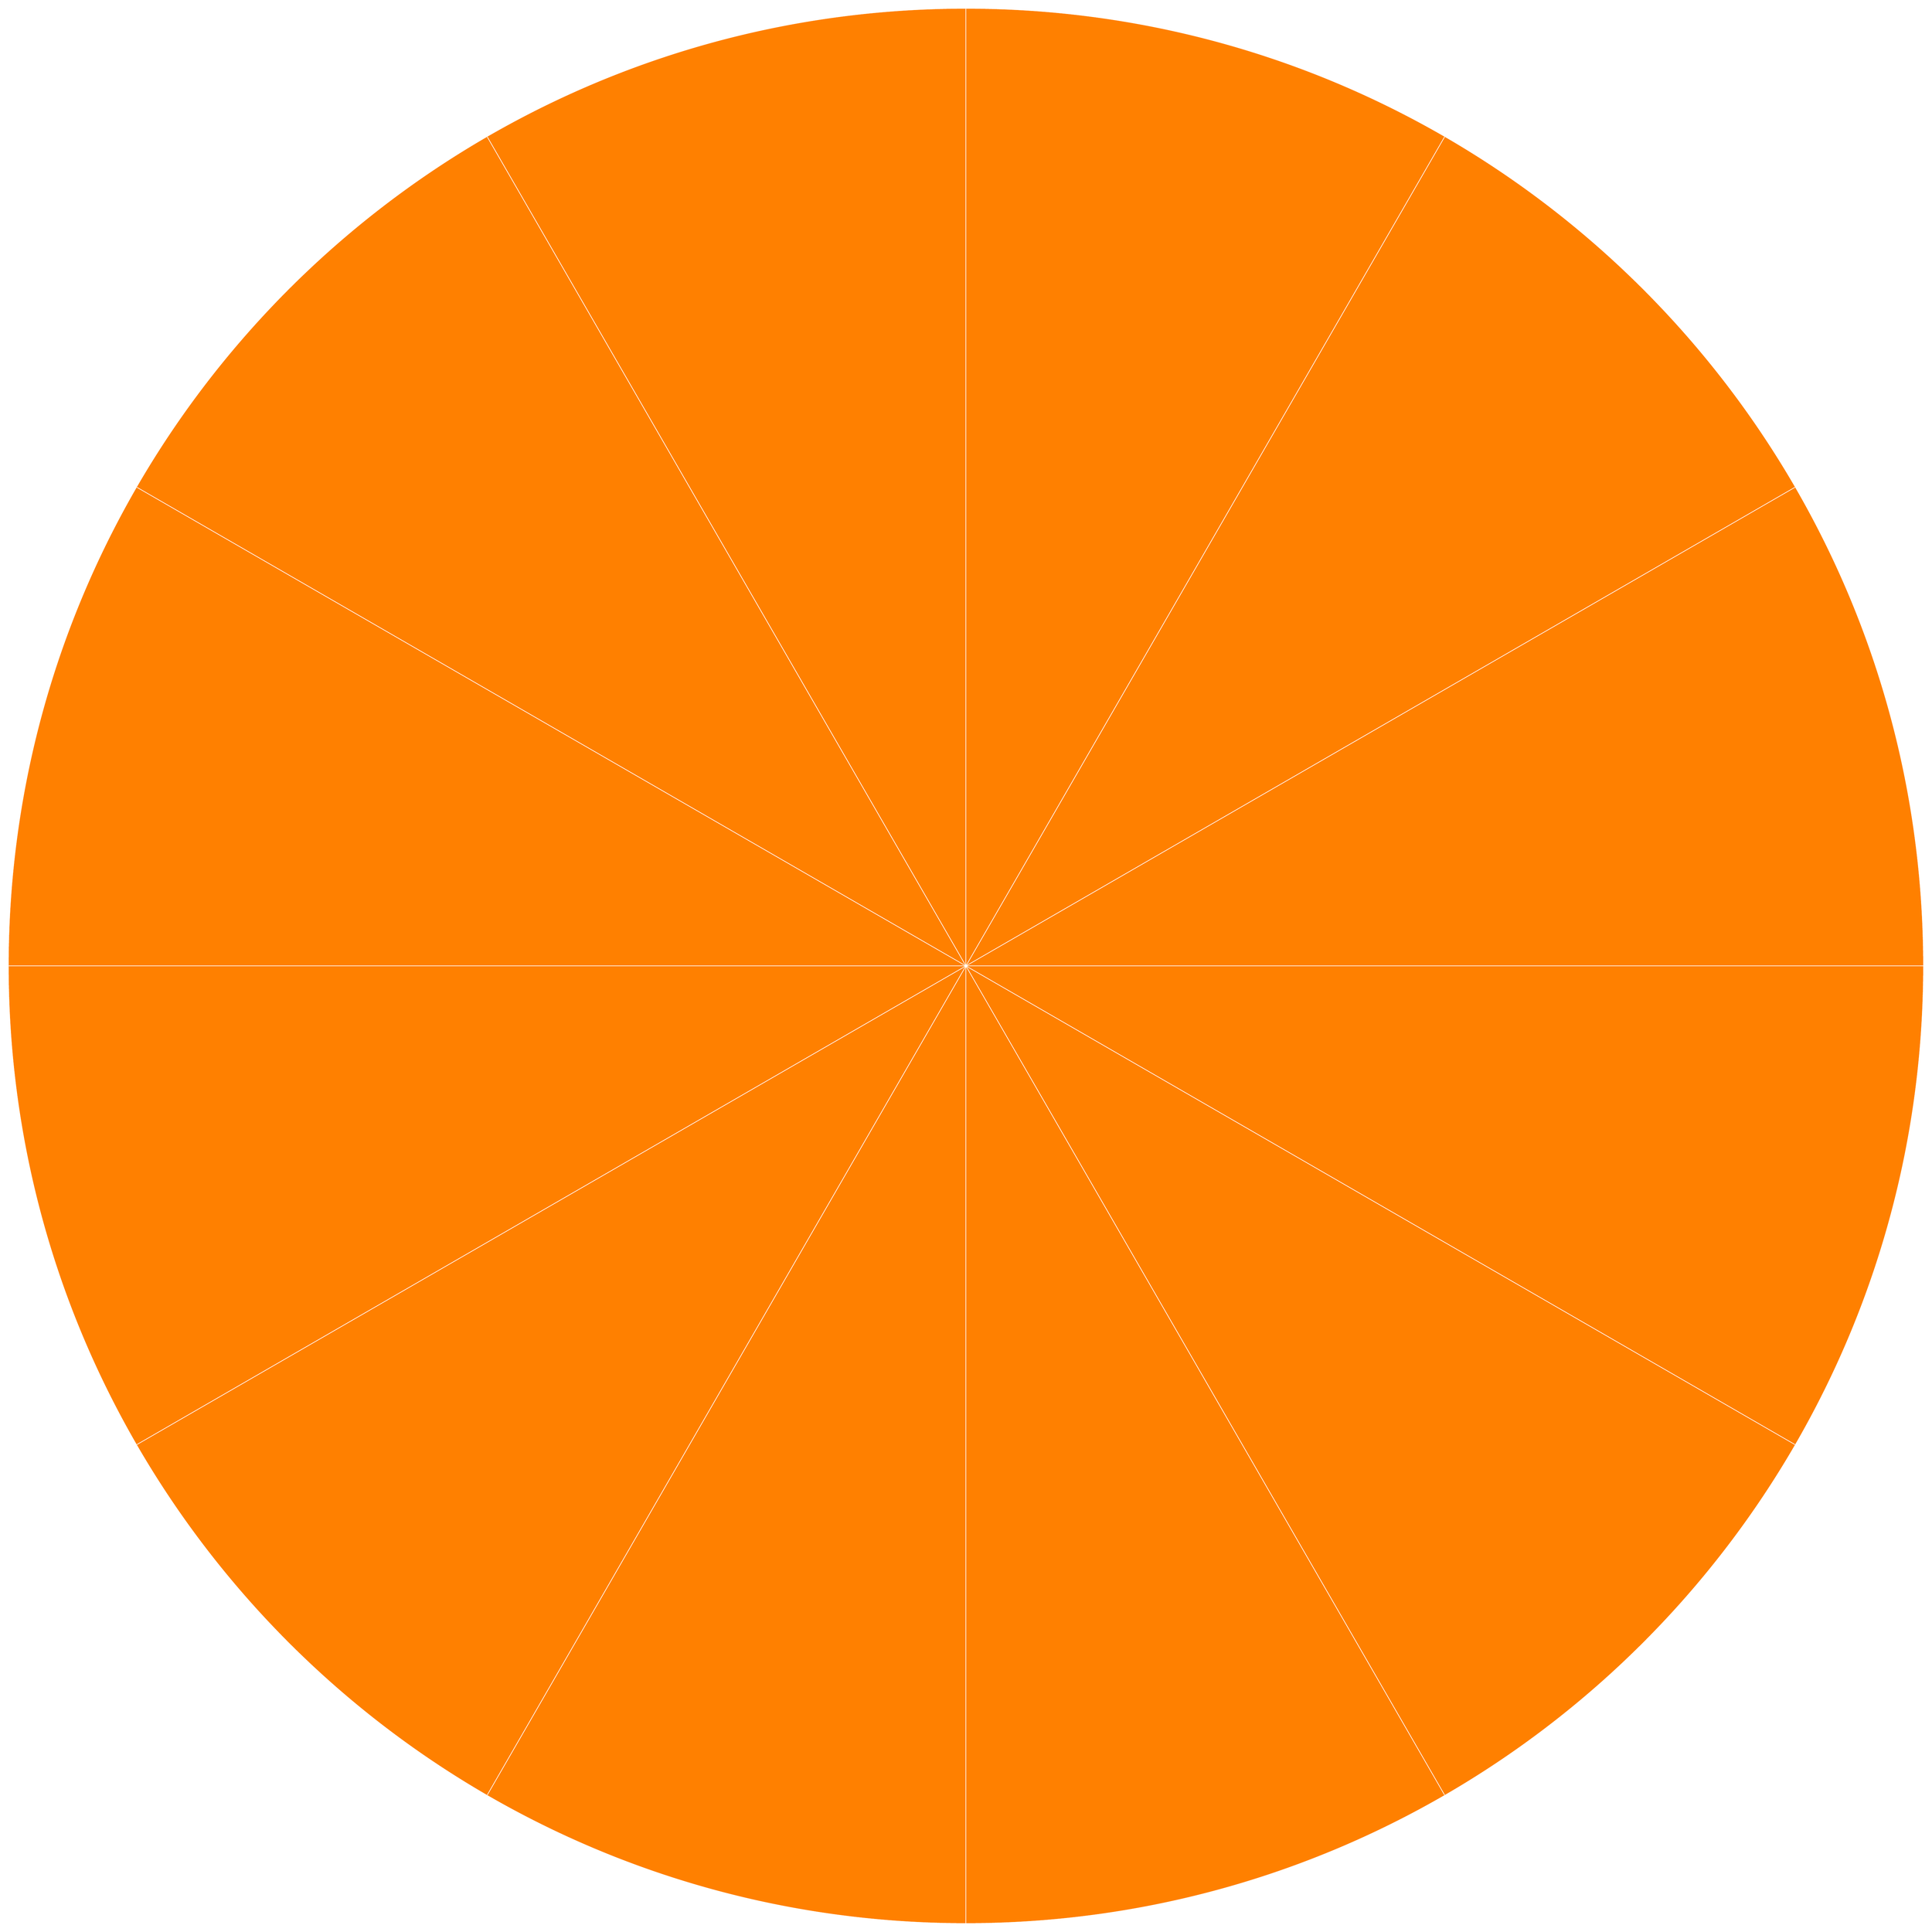
\begin{tikzpicture}
\fill[orange] (0,0) circle (40);
\foreach \x in {0,30,...,360} \draw[line width =.25mm, white] (0,0)--(\x:40);
\end{tikzpicture}
&
\begin{tikzpicture}
\draw (0,0) circle (40);
\foreach \x in {0,36,...,360} \draw[line width =.25mm] (0,0)--(\x:40);
\end{tikzpicture}
\end{longtable}



\noindent {\bf Atividade 12}
\vspace{.2cm}

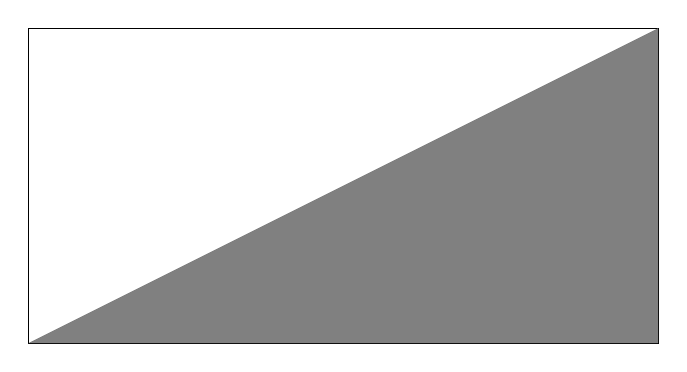
\begin{tikzpicture}[scale=2, x=1cm,y=1cm]
 \draw (0,0) rectangle (4,2);
 \fill[gray] (0,0) -- (4,2) -- (4,0) -- cycle;
\end{tikzpicture}

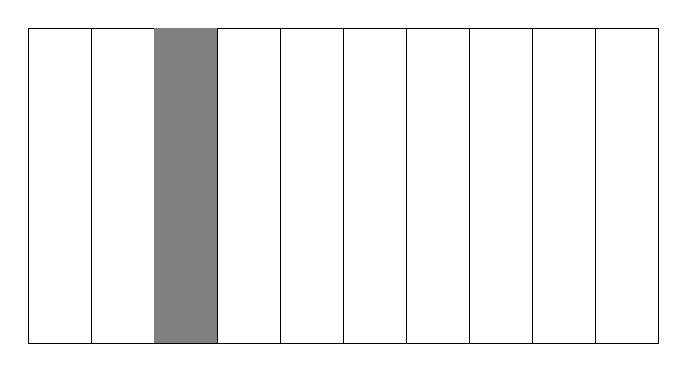
\begin{tikzpicture}[scale=2, x=1cm,y=1cm]
 \draw (0,0) rectangle (4,2);
 \foreach \n in {0.4,0.8,1.2,...,3.2,3.6}{
 \draw (\n,0) -- (\n,2);}
 \fill[gray] (0.8,0) -- (0.8,2) -- (1.2,2) -- (1.2,0) -- cycle;
\end{tikzpicture}
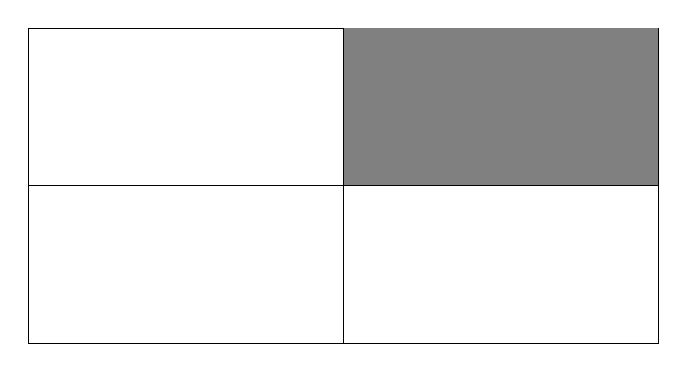
\begin{tikzpicture}[scale=2, x=1cm,y=1cm]
 \draw (0,0) rectangle (4,2);
 \fill[gray] (2,1) rectangle (4,2);
 \draw (0,1) -- (4,1);
 \draw (2,0) -- (2,2);
 \end{tikzpicture}

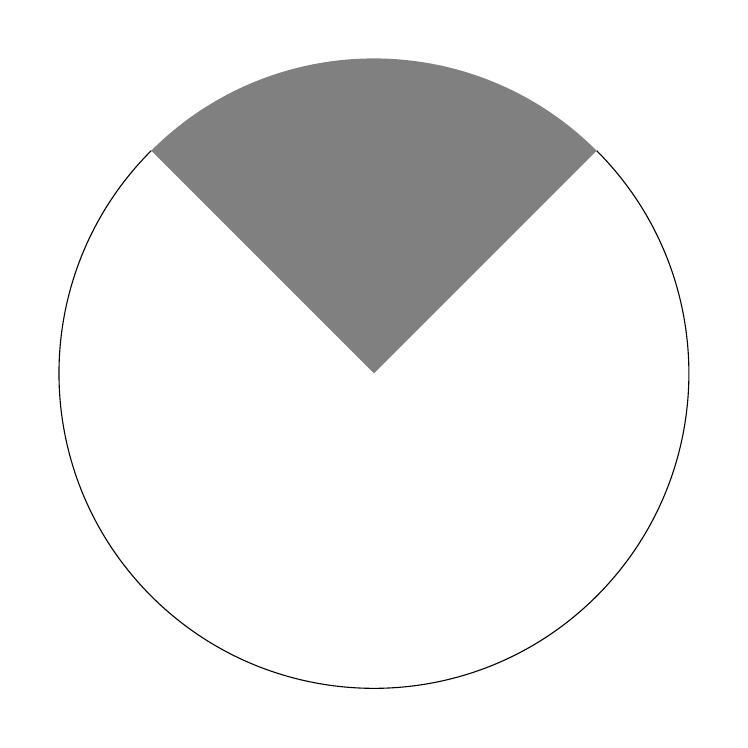
\begin{tikzpicture}[scale=2, x=1cm,y=1cm]
 \fill[gray] (45:2) arc (45:135:2) -- (0,0) -- cycle;
 \draw (135:2) arc (135:405:2);
\end{tikzpicture}
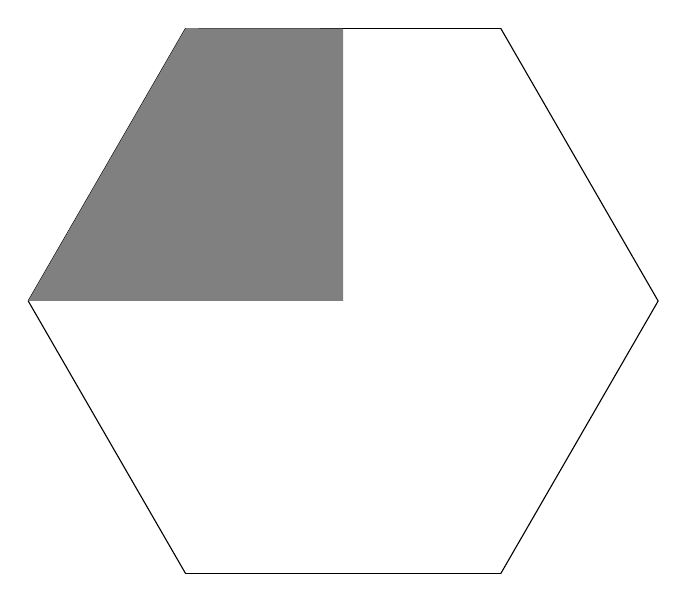
\begin{tikzpicture}[scale=2,x=1cm,y=1cm]
 \foreach \x in {0,60,...,300}{
 \draw (\x:2) -- (\x +60: 2);}
\fill[gray] (-2,0) -- (0,0) -- (0,1.73) -- (120:2) -- cycle;
\end{tikzpicture}

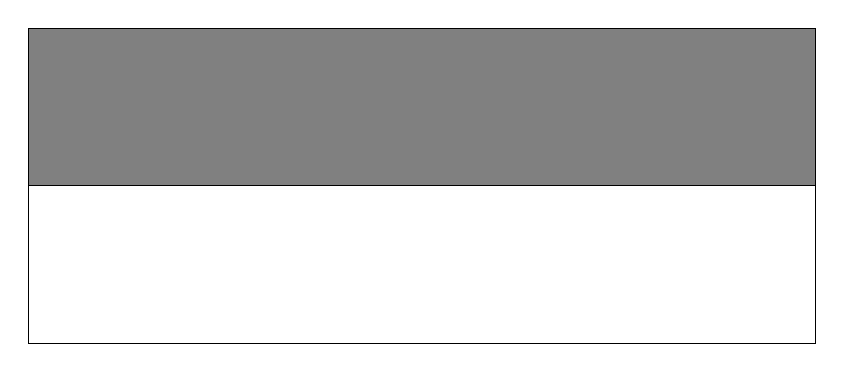
\begin{tikzpicture}[scale=2,x=1cm,y=1cm]
 \draw (0,0) rectangle (5,1);
 \draw[fill=gray] (0,1) rectangle (5,2);
\end{tikzpicture}


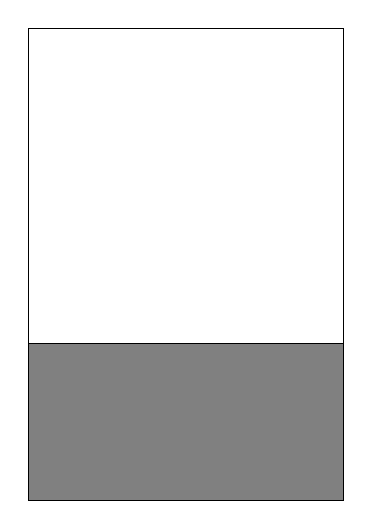
\begin{tikzpicture}[scale=2,x=1cm,y=1cm]
 \draw[fill=gray] (0,0) rectangle (2,1);
 \draw (0,1) rectangle (2,3);
\end{tikzpicture} 
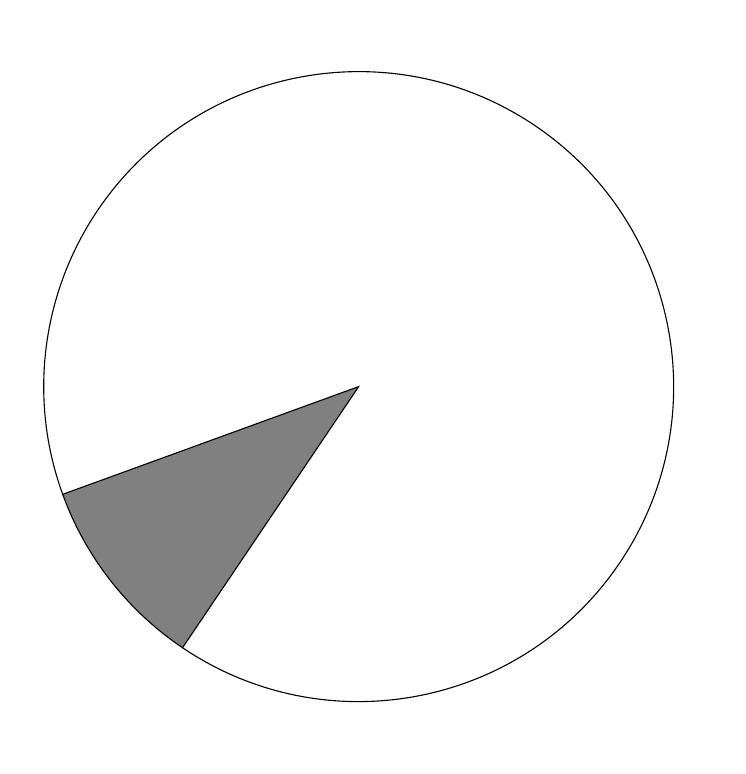
\begin{tikzpicture}[scale=2,x=1cm,y=1cm]
 \draw[fill=gray] (200:2) arc (200:236:2) -- (0,0) -- cycle;
 \draw (236:2) arc (236:560:2);
\end{tikzpicture} 

%i)
\begin{tikzpicture}[scale=2,x=1cm,y=1cm]
 \draw[line width=2pt] (-1,0) arc (180:270:1);
 \draw (0,-1) arc (270:360:1) -- (1,0) arc (180:0:1);
 \end{tikzpicture}
%j) paralelepípedo
\begin{tikzpicture}[scale=2,x=1cm,y=1cm]
    \pic [fill=gray] at (0,0) {annotated cuboid={width=5, height=10, depth=10}};
    \pic [fill=white] at (4.5,0) {annotated cuboid={width=45, height=10, depth=10}};
    \end{tikzpicture}


%l)
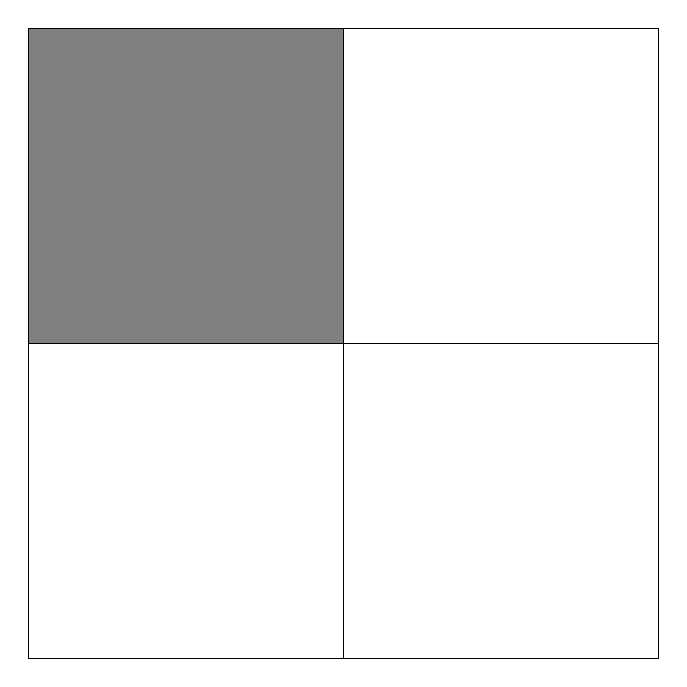
\begin{tikzpicture}[scale=2,x=1cm,y=1cm]
 \draw[fill=gray] (0,2) rectangle (2,4);
 \draw (0,0) rectangle (2,2);
 \draw (2,0) rectangle (4,2);
 \draw (2,2) rectangle (4,4);
 \end{tikzpicture} 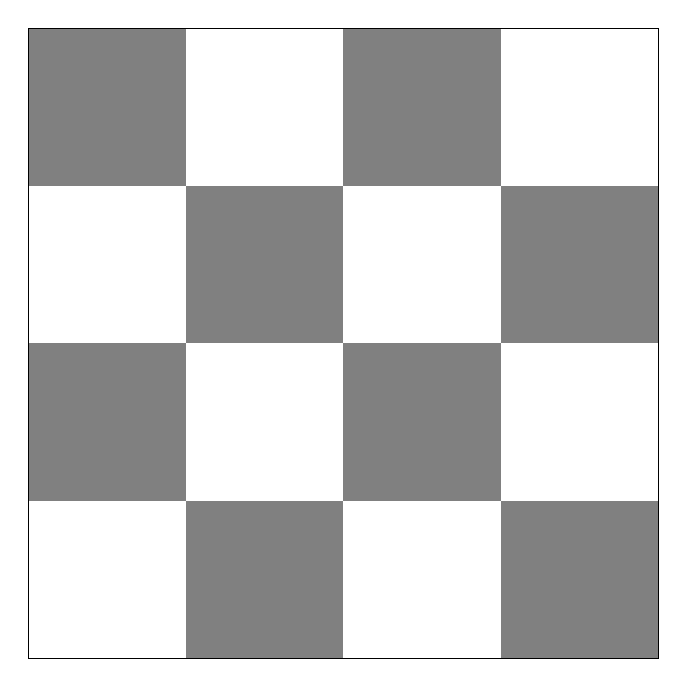
\begin{tikzpicture}[scale=2,x=1cm,y=1cm]
 \fill[gray] (1,0) rectangle (2,1);
 \fill[gray] (3,0) rectangle (4,1);
 \fill[gray] (0,1) rectangle (1,2);
 \fill[gray] (2,1) rectangle (3,2);
 \fill[gray] (1,2) rectangle (2,3);
 \fill[gray] (3,2) rectangle (4,3);
 \fill[gray] (0,3) rectangle (1,4);
 \fill[gray] (2,3) rectangle (3,4);
 \draw (0,0) rectangle (4,4);
\end{tikzpicture}


\section{Licao 2}

\noindent {\bf Atividade 1}
\vspace{.2cm}


\begin{tikzpicture}[scale=2]
\draw[fill=gray] (0,0) rectangle (60,20);
\end{tikzpicture}

\noindent {\bf Atividade 2}
\vspace{.2cm}

\begin{tikzpicture}[scale=2]
  \draw (0,0) rectangle (60,30);
 \end{tikzpicture}

 
\noindent {\bf Atividade 17}
\vspace{.2cm}


\begin{tikzpicture}%[scale=.5]
\draw[fill=gray] (0,0) rectangle (60,12);
    \end{tikzpicture}

\begin{tikzpicture}%[scale=.5]
\draw[fill=light] (0,0) rectangle (60,12);
\draw (30,0) -- (30,12);
\node at (15,6) {{\small $\frac{1}{2}$}};
\node at (45,6) {{\small $\frac{1}{2}$}};
\end{tikzpicture}
    
   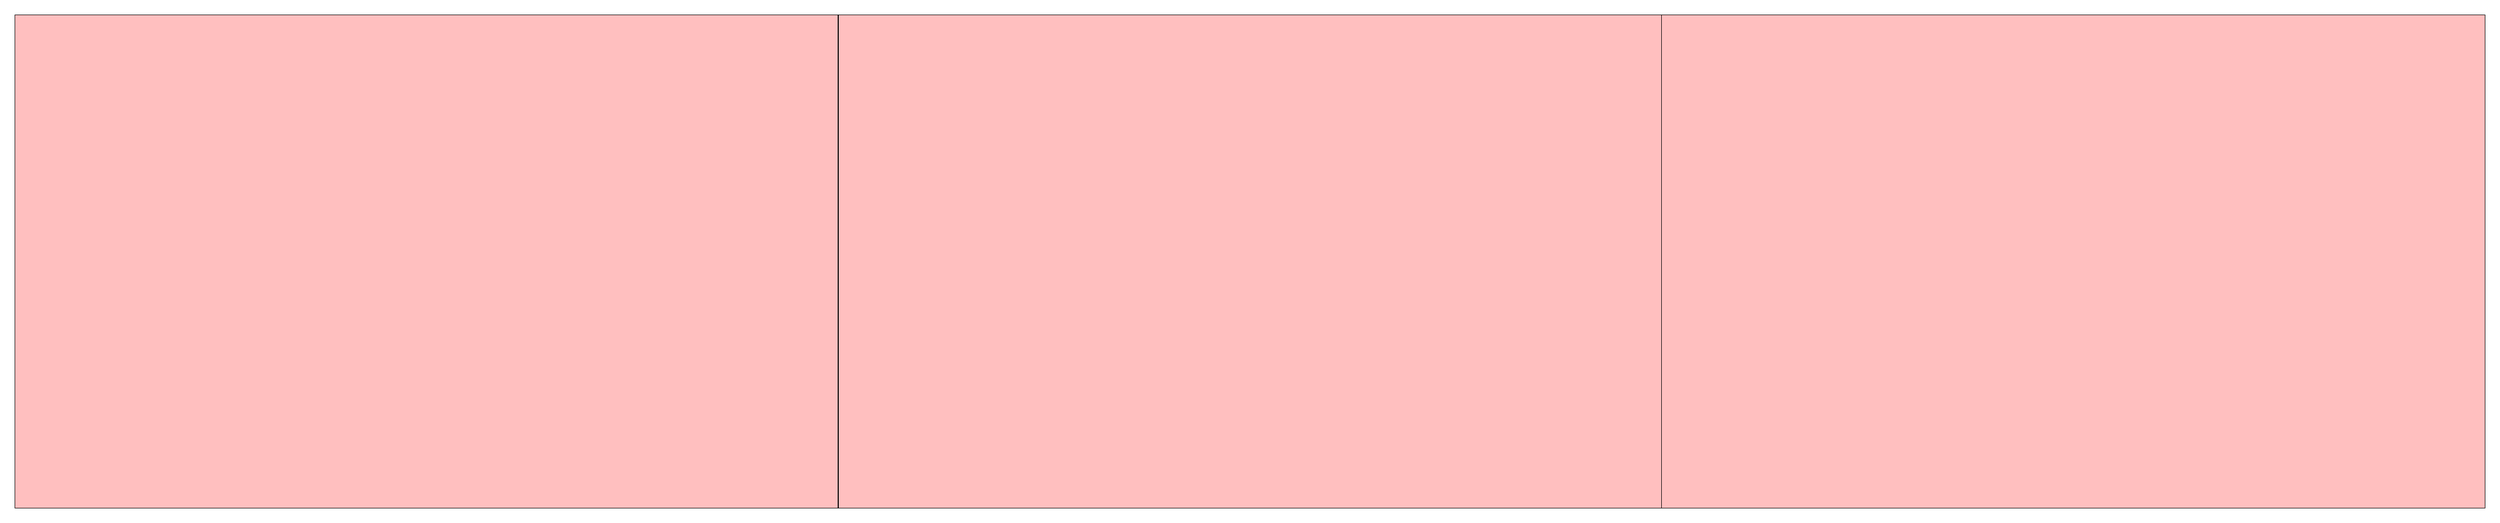
\begin{tikzpicture}%[scale=.5]
\draw[fill=pink] (0,0) rectangle (60,12);
\foreach \x in {1,2} \draw (\x*60/3,0) -- (\x*60/3,12);
    \end{tikzpicture}        
    
      \begin{tikzpicture}%[scale=.5]
\draw[fill=special] (0,0) rectangle (60,12);
\foreach \x in {1,2,3} \draw (\x*60/4,0) -- (\x*60/4,12);
    \end{tikzpicture}        
    
   \begin{tikzpicture}%[scale=.5]
\draw[fill=attention] (0,0) rectangle (60,12);
\foreach \x in {1,...,4} \draw (\x*60/5,0) -- (\x*60/5,12);
    \end{tikzpicture}        
    
   \begin{tikzpicture}%[scale=.5]
\draw[fill=common] (0,0) rectangle (60,12);
\foreach \x in {1,...,5} \draw (\x*60/6,0) -- (\x*60/6,12);
    \end{tikzpicture}        
    
    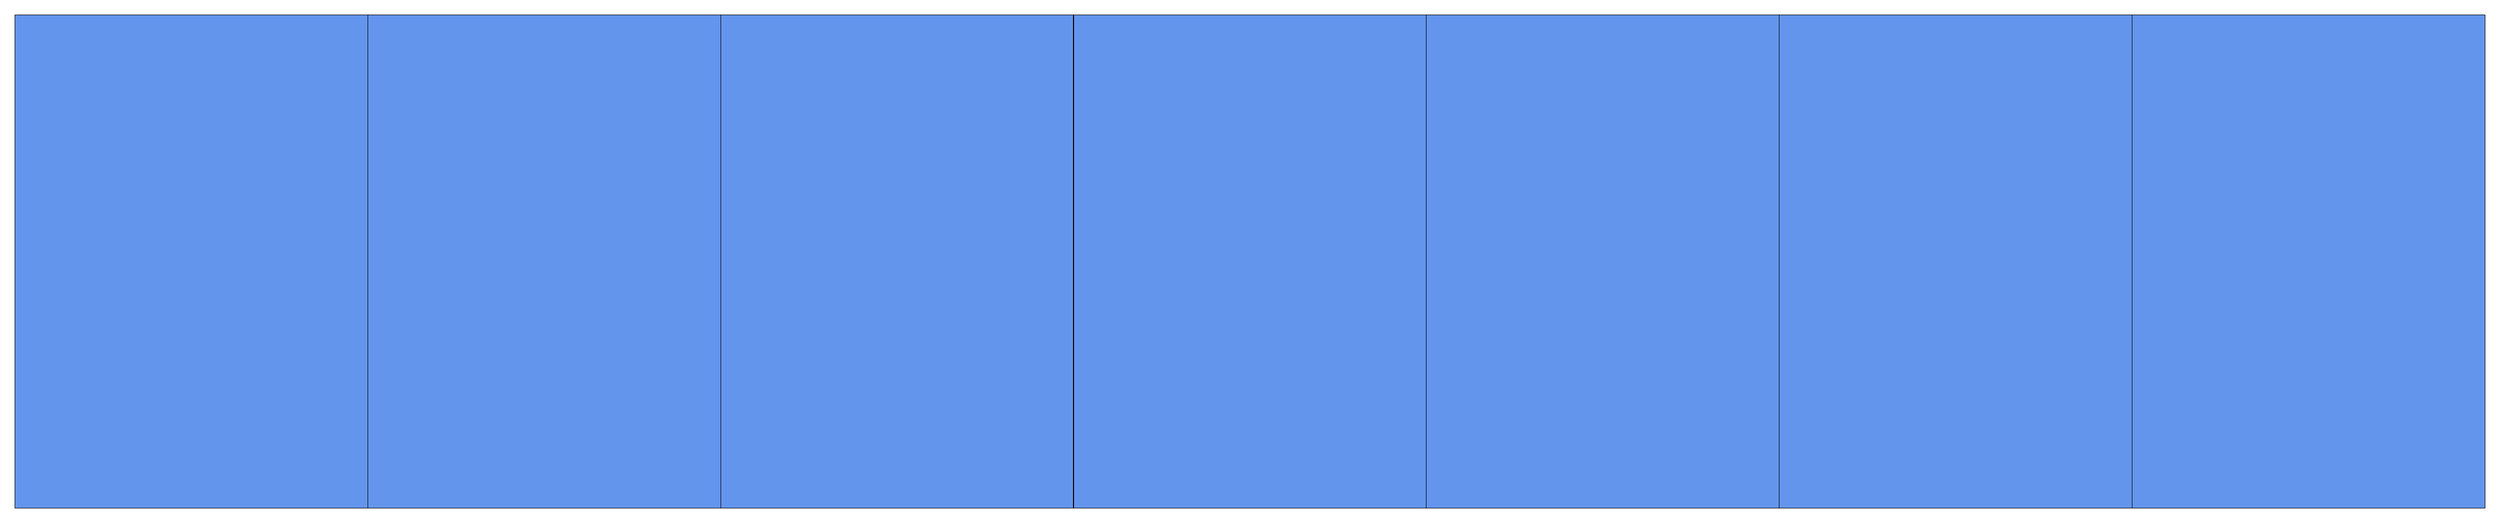
\begin{tikzpicture}%[scale=.5]
\draw[fill=CornflowerBlue] (0,0) rectangle (60,12);
\foreach \x in {1,...,6} \draw (\x*60/7,0) -- (\x*60/7,12);
    \end{tikzpicture}        
    
   \begin{tikzpicture}%[scale=.5]
\draw[fill=dark] (0,0) rectangle (60,12);
\foreach \x in {1,...,7} \draw (\x*60/8,0) -- (\x*60/8,12);
    \end{tikzpicture}        
    
   \begin{tikzpicture}%[scale=.5]
\draw[fill=Fuchsia] (0,0) rectangle (60,12);'
\foreach \x in {1,...,8} \draw (\x*60/9,0) -- (\x*60/9,12);
    \end{tikzpicture}        
    
 \begin{tikzpicture}%[scale=.5]   
 \draw[fill=NavyBlue] (0,0) rectangle (60,12);
 \foreach \x in {1,...,9} \draw (\x*60/10,0) -- (\x*60/10,12);
     \end{tikzpicture}        
    
\begin{tikzpicture}%[scale=.5]   
    \draw[fill=BlueViolet] (0,0) rectangle (60,12);
\foreach \x in {1,...,15} \draw (\x*60/16,0) -- (\x*60/16,12);
    \end{tikzpicture}        
 
 
\section{Licao 3}

\noindent {\bf Atividade 6}
\vspace{.2cm}

\begin{tikzpicture}[x=115mm,y=115mm]
\draw[fill=common] (0,-.15) rectangle (1.2,.15);
\draw (0,0) -- (1.2,0) ; %edit here for the axis
\draw (1,3pt) -- (1,-3pt) node[below] {1};
\node at (.03,-.05) {0};
\end{tikzpicture} 

\noindent {\bf Atividade 7} 
\vspace{.2cm}

\begin{tikzpicture}
 \draw[fill=gray] (0,0) rectangle (110,15);
\end{tikzpicture}

\pagebreak

\section{Licao 4}

\noindent {\bf Atividade 2} 
 \vspace{.2cm}
 
\begin{tikzpicture}[scale=1.5]
 \fill[gray] (0,0) rectangle (80,18);
 \draw (0,0) rectangle (80,60);
 \foreach \x in {6,12,...,54} \draw (0,\x) -- (80,\x);
\end{tikzpicture}

\noindent {\bf Atividade 4} 
\vspace{.2cm}

\begin{tikzpicture}
\draw (0,0) circle (40);
\foreach \x in {30,150,270} \draw[line width =1mm] (0,0)--(\x:40);
\end{tikzpicture}
\begin{tikzpicture}
\draw (0,0) circle (40);
\foreach \x in {30,60,...,360} \draw[line width =.2mm] (0,0)--(\x:40);
\draw[line width =1mm] (0,0)--(0:40);
\draw[line width =1mm] (0,0)--(120:40);
\draw[line width =1mm] (0,0)--(240:40);
\end{tikzpicture}
\clearpage

\noindent {\bf Atividade 5} 
\vspace{.2cm}

\begin{center}
 \begin{tikzpicture}[scale=2.8]
  \draw[fill=gray] (20,0) arc (0:240:20) -- (0,0)--cycle;
  \draw (0,0) circle (20);
 \end{tikzpicture}
\end{center}

\noindent {\bf Atividade 6} 
\vspace{.2cm}

\begin{tikzpicture}[scale=2]
\draw[fill=light] (0,0) rectangle (60,12);
\draw (30,0) -- (30,12);
    \end{tikzpicture}
    
   \begin{tikzpicture}[scale=2]
\draw[fill=pink] (0,0) rectangle (60,12);
\foreach \x in {1,2} \draw (\x*60/3,0) -- (\x*60/3,12);
    \end{tikzpicture}        
    
      \begin{tikzpicture}[scale=2]
\draw[fill=special] (0,0) rectangle (60,12);
\foreach \x in {1,2,3} \draw (\x*60/4,0) -- (\x*60/4,12);
    \end{tikzpicture}        
    
   \begin{tikzpicture}[scale=2]
\draw[fill=attention] (0,0) rectangle (60,12);
\foreach \x in {1,...,4} \draw (\x*60/5,0) -- (\x*60/5,12);
    \end{tikzpicture}        
    
   \begin{tikzpicture}[scale=2]
\draw[fill=common] (0,0) rectangle (60,12);
\foreach \x in {1,...,5} \draw (\x*60/6,0) -- (\x*60/6,12);
    \end{tikzpicture}        
    
    \begin{tikzpicture}[scale=2]
\draw[fill=CornflowerBlue] (0,0) rectangle (60,12);
\foreach \x in {1,...,6} \draw (\x*60/7,0) -- (\x*60/7,12);
    \end{tikzpicture}        
    
   \begin{tikzpicture}[scale=2]
\draw[fill=dark] (0,0) rectangle (60,12);
\foreach \x in {1,...,7} \draw (\x*60/8,0) -- (\x*60/8,12);
    \end{tikzpicture}        
    
   \begin{tikzpicture}[scale=2]
\draw[fill=Fuchsia] (0,0) rectangle (60,12);'
\foreach \x in {1,...,8} \draw (\x*60/9,0) -- (\x*60/9,12);
    \end{tikzpicture}        
    
 \begin{tikzpicture}[scale=2]   
 \draw[fill=NavyBlue] (0,0) rectangle (60,12);
 \foreach \x in {1,...,9} \draw (\x*60/10,0) -- (\x*60/10,12);
     \end{tikzpicture}        
    
\begin{tikzpicture}[scale=2]   
    \draw[fill=BlueViolet] (0,0) rectangle (60,12);
\foreach \x in {1,...,15} \draw (\x*60/16,0) -- (\x*60/16,12);
    \end{tikzpicture}        
    
\begin{tikzpicture}[x=1mm, y=1mm, scale=1.2]
% Fita principal (metade cinza, metade branca)
\draw (0,0) rectangle (100,10);
\draw[fill=lightgray] (0,0) rectangle (100/2,10);
\end{tikzpicture}

\pagebreak
 
\noindent {\bf Atividade 20}
\vspace{.2cm}

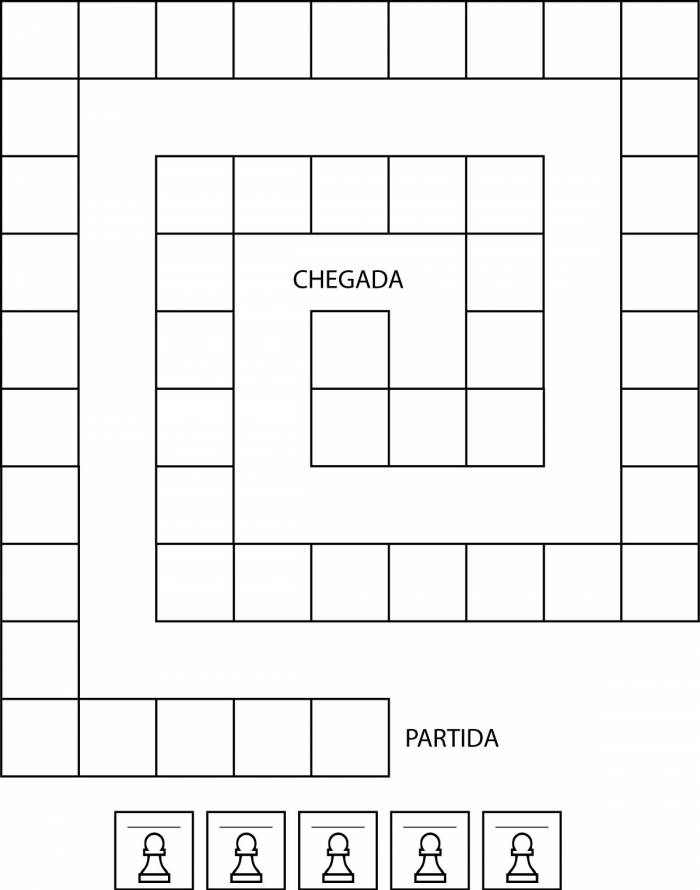
\includegraphics[scale=.4]{../media/cap1/secoes/pngs_licao_01/caminho-reproducao-01.jpg}
 
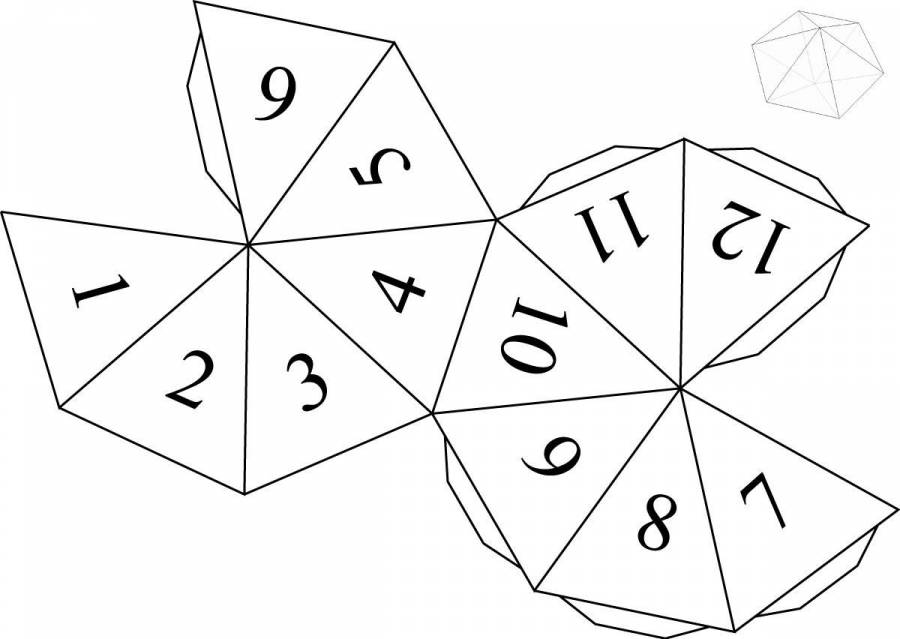
\includegraphics[scale=.4]{../media/cap1/secoes/pngs_licao_01/caminho-reproducao-02.jpg}

%\clearpage
\section{Lição 5}
 
\noindent {\bf Atividade 4}
\vspace{.2cm}

\begin{tikzpicture}[scale=2]
\foreach \x in {0,30,...,150}{ \draw (\x:20) -- (\x:-20);}
\draw (0,0) circle (20);
\end{tikzpicture}
